%%%%%%%%%%%%%%%%%%%%%%%%%%%%%%%%%%%%%%%%%%%%%%%%%%%%%%%%%%%%%%%%%%%%%%%%%%%%%%%
%                       CARREGA DE LA CLASSE DE DOCUMENT                      %
%                                                                             %
% Les opcions admissibles son:                                                %
%      12pt / 11pt            (cos dels tipus de lletra; no feu servir 10pt)  %
%                                                                             %
% catalan/spanish/english     (llengua principal del treball)                 %
%                                                                             % 
% french/italian/german...    (si necessiteu fer servir alguna altra llengua) %
%                                                                             %
% listoffigures               (El document inclou un Index de figures)        %
% listoftables                (El document inclou un Index de taules)         %
% listofquadres               (El document inclou un Index de quadres)        %
% listofalgorithms            (El document inclou un Index d'algorismes)      %
%                                                                             %
%%%%%%%%%%%%%%%%%%%%%%%%%%%%%%%%%%%%%%%%%%%%%%%%%%%%%%%%%%%%%%%%%%%%%%%%%%%%%%%
\PassOptionsToPackage{table}{xcolor}

\documentclass[11pt,catalan,listoffigures,listoftables]{tfgetsinf}
\renewcommand{\labelitemii}{$\diamond$}

\setlength{\arrayrulewidth}{1mm}
\setlength{\tabcolsep}{10pt}
\renewcommand{\arraystretch}{1.3}
 
\newcolumntype{s}{>{\columncolor[HTML]{AAACED}} p{3cm}}
 
\arrayrulecolor[HTML]{000000}

%%%%%%%%%%%%%%%%%%%%%%%%%%%%%%%%%%%%%%%%%%%%%%%%%%%%%%%%%%%%%%%%%%%%%%%%%%%%%%%
%                     CODIFICACIO DEL FITXER FONT                             %
%                                                                             %
%    windows fa servir normalment 'ansinew'                                   %
%    amb linux es possible que siga 'latin1' o 'latin9'                       %
%    Pero el mes recomanable es fer servir utf8 (unicode 8)                   %
%                                          (si el vostre editor ho permet)    % 
%%%%%%%%%%%%%%%%%%%%%%%%%%%%%%%%%%%%%%%%%%%%%%%%%%%%%%%%%%%%%%%%%%%%%%%%%%%%%%%
\usepackage{hyperref}
\usepackage{float}
\usepackage{lmodern,textcomp}
\usepackage[utf8]{inputenc} 
\usepackage{listings}
\definecolor{forestgreen}{RGB}{34,139,34}
\definecolor{costumyellow}{RGB}{255,185,1}
\definecolor{lightgray}{rgb}{.9,.9,.9}
\definecolor{darkgray}{rgb}{.4,.4,.4}
\definecolor{purple}{rgb}{0.65, 0.12, 0.82}

\lstdefinelanguage{JavaScript}{
  keywords={typeof, new, true, false, catch, function, return, null, catch, switch, var, if, in, while, do, else, case, break},
  keywordstyle=\color{blue}\bfseries,
  ndkeywords={class, export, boolean, throw, implements, import, this},
  ndkeywordstyle=\color{darkgray}\bfseries,
  identifierstyle=\color{black},
  sensitive=false,
  comment=[l]{//},
  morecomment=[s]{/*}{*/},
  commentstyle=\color{purple}\ttfamily,
  stringstyle=\color{red}\ttfamily,
  morestring=[b]',
  morestring=[b]"
}

\lstset{
   language=JavaScript,
   backgroundcolor=\color{lightgray},
   extendedchars=true,
   basicstyle=\footnotesize\ttfamily,
   showstringspaces=false,
   showspaces=false,
   numbers=right,
   numberstyle=\footnotesize,
   numbersep=9pt,
   tabsize=2,
   breaklines=true,
   showtabs=false,
   captionpos=b
}

%%%%%%%%%%%%%%%%%%%%%%%%%%%%%%%%%%%%%%%%%%%%%%%%%%%%%%%%%%%%%%%%%%%%%%%%%%%%%%%
%                        ALTRES PAQUETS I DEFINICIONS                         %
%                                                                             %
% Carregueu aci els paquets que necessiteu i declareu les comandes i entorns  %
%                                          (aquesta seccio pot ser buida)     %
%%%%%%%%%%%%%%%%%%%%%%%%%%%%%%%%%%%%%%%%%%%%%%%%%%%%%%%%%%%%%%%%%%%%%%%%%%%%%%%



%%%%%%%%%%%%%%%%%%%%%%%%%%%%%%%%%%%%%%%%%%%%%%%%%%%%%%%%%%%%%%%%%%%%%%%%%%%%%%%
%                        DADES DEL TREBALL                                    %
%                                                                             %
% titol, alumne, tutor i curs academic                                        %
%%%%%%%%%%%%%%%%%%%%%%%%%%%%%%%%%%%%%%%%%%%%%%%%%%%%%%%%%%%%%%%%%%%%%%%%%%%%%%%

\title{Implementació de xarxa social per a persones amb diversitat funcional}
\author{David Aleu Moseguí}
\tutor{Xavier Burgués Illa}
\curs{2016-2017}

%%%%%%%%%%%%%%%%%%%%%%%%%%%%%%%%%%%%%%%%%%%%%%%%%%%%%%%%%%%%%%%%%%%%%%%%%%%%%%%
%                     PARAULES CLAU/PALABRAS CLAVE/KEY WORDS                  %
%                                                                             %
% Independentment de la llengua del treball, s'hi han d'incloure              %
% les paraules clau i el resum en els tres idiomes                            %
%%%%%%%%%%%%%%%%%%%%%%%%%%%%%%%%%%%%%%%%%%%%%%%%%%%%%%%%%%%%%%%%%%%%%%%%%%%%%%%

\keywords{????, ?????????, ????, ?????????????????} % Paraules clau 
         {?????, ???, ???????????????}              % Palabras clave
         {?????, ????? ?????, ?????????????}        % Key words

%%%%%%%%%%%%%%%%%%%%%%%%%%%%%%%%%%%%%%%%%%%%%%%%%%%%%%%%%%%%%%%%%%%%%%%%%%%%%%%
%                              INICI DEL DOCUMENT                             %
%%%%%%%%%%%%%%%%%%%%%%%%%%%%%%%%%%%%%%%%%%%%%%%%%%%%%%%%%%%%%%%%%%%%%%%%%%%%%%%

\begin{document}

%%%%%%%%%%%%%%%%%%%%%%%%%%%%%%%%%%%%%%%%%%%%%%%%%%%%%%%%%%%%%%%%%%%%%%%%%%%%%%%
%              RESUMS DEL TFG EN VALENCIA, CASTELLA I ANGLES                  %
%%%%%%%%%%%%%%%%%%%%%%%%%%%%%%%%%%%%%%%%%%%%%%%%%%%%%%%%%%%%%%%%%%%%%%%%%%%%%%%

\begin{abstract}
????
\end{abstract}
\begin{abstract}[spanish]
????
\end{abstract}
\begin{abstract}[english]
????
\end{abstract}

%%%%%%%%%%%%%%%%%%%%%%%%%%%%%%%%%%%%%%%%%%%%%%%%%%%%%%%%%%%%%%%%%%%%%%%%%%%%%%%
%                              CONTINGUT DEL TREBALL                          %
%%%%%%%%%%%%%%%%%%%%%%%%%%%%%%%%%%%%%%%%%%%%%%%%%%%%%%%%%%%%%%%%%%%%%%%%%%%%%%%

\mainmatter

%%%%%%%%%%%%%%%%%%%%%%%%%%%%%%%%%%%%%%%%%%%%%%%%%%%%%%%%%%%%%%%%%%%%%%%%%%%%%%%
%                                  INTRODUCCIO                                %
%%%%%%%%%%%%%%%%%%%%%%%%%%%%%%%%%%%%%%%%%%%%%%%%%%%%%%%%%%%%%%%%%%%%%%%%%%%%%%%

\chapter{Introducció i Contextualització}

\section{Context}

\subsection{Introducció}

Aquest projecte es realitza com a Treball Final de Grau de modalitat A, dels estudis de Grau en Enginyeria Informàtica, especialitat en Enginyeria del Software, a la Facultat d’Informàtica de Barcelona (Universitat Politècnica de Catalunya).
El projecte en qüestió, tracta en desenvolupar una xarxa social per a persones amb diversitat funcional de dèficit cognitiu, per tal de facilitar les comunicacions que puguin tindre entre ells a través d’internet.

\subsection{Stakeholders}

Com en tots els projectes, hi haurà unes parts interessades (o stakeholders), les quals aportaran diferents objectius i visions. En aquesta secció, definirem i explicarem quines són les parts interessades i que aportaran cadascuna d’elles en el nostre projecte.
\begin{itemize}
	\item \textbf{Director del projecte:} \\El director del projecte és Xavier Burgués Illa, i serà l’encarregat de guiar i supervisar tota la feina fet per l’autor del projecte.
	\item \textbf{Equip desenvolupador del sistema:} \\És el que s’encarregarà de tirar el projecte endavant, des del disseny de l’aplicació a la codificació. En un projecte normal, hi hauria diferents persones interpretant diferents rols (cap de projecte, analista, dissenyador, programador, etc.), però en aquest cas, l’autor del projecte serà qui exercirà cadascun d’aquests rols.
	\item \textbf{Usuaris:} \\ Els usuaris potencials del sistema són aquelles persones amb diversitat funcional de dèficit cognitiu de grau mitja/baix, els quals utilitzaran el sistema per comunicar-se entre ells de manera similar a Facebook. \\Per altra banda, també hi haurà usuaris que tinguin relació en aquest àmbit, ho sigui, professionals especialitzats (logopedes, psicoterapeutes, etc.). \\Pel que fa a la resta de gent, no tindrien accés a la xarxa social.
	\item \textbf{UTAC:} \\La UTAC (Unitat de Tècniques Augmentatives de Comunicació) és un servei extern a la Facultat de Psicologia de la UB (Universitat de Barcelona), la qual ajudarà a l’autor del projecte a entendre com s’ha de dissenyar la interfície gràfica de la xarxa social perquè els seus usuaris s’hi puguin moure més còmodament.
	\item \textbf{Competència:}\\Indirectament, la competència també actua com a part interessada. Avui en dia existeixen moltes xarxes socials, com ara Facebook i Twitter, les quals no tenen implementades diferents capes gràfiques adaptades per a cadascun dels usuaris. Per tant, aquestes xarxes socials podrien representar una competència en el projecte actual.
\end{itemize}

%\section{Notes bibliografiques} %%%%% Opcional

%????? ????????????? ????????????? ????????????? ????????????? ?????????????

%%%%%%%%%%%%%%%%%%%%%%%%%%%%%%%%%%%%%%%%%%%%%%%%%%%%%%%%%%%%%%%%%%%%%%%%%%%%%%%
%                         CAPITOLS (tants com calga)                          %
%%%%%%%%%%%%%%%%%%%%%%%%%%%%%%%%%%%%%%%%%%%%%%%%%%%%%%%%%%%%%%%%%%%%%%%%%%%%%%%

\section{Estat de l’Art}

\subsection{Contextualització}

Una xarxa social és una estructura social composta per individus que estan lligats per un o més tipus d’interdependència. Dins del que serien les xarxes socials, podem trobar-ne de dos tipus:

\begin{itemize}
	\item \textbf{Xarxes Socials Analògiques:} \\Formades per grups de persones relacionades entre si, i que es desenvolupen sense sistemes electrònics.
	\item \textbf{Xarxes Socials Digitals:} \\Formades per grups de persones relacionades entre si, i que es desenvolupen utilitzant sistemes electrònics.
\end{itemize}  
A més, dins de les xarxes socials digitals, també tenim dos grups:
\begin{itemize}
	\item \textbf{Xarxes Socials Digitals Horitzontals:} \\Dirigides a tot tipus d’usuaris i sense cap temàtica concreta. Facebook i Twitter en serien un exemple.
	\item \textbf{Xarxes Socials Digitals Verticals: } \\Es basen en un tema concret. Alguns exemples serien LinkedIn (xarxa social amb temàtica professional) o Pinterest (xarxa social amb temàtica d’oci fotogràfic).
\end{itemize}  
Pel que fa al naixement de les xarxes socials, és una mica complex d’explicar. Des de fa molt de temps que les persones han creat comunitat per xerrar de temes que tenen en comú, però fins no fa gaires anys, no es va traslladar la idea de portar-ho a la xarxa. Des del punt de vista de la comunicació a través d’internet, podríem dir que el seu naixement és el 1971, en el moment en què s’aconsegueix enviar un correu electrònic entre dos ordinadors. El 1978, neix el BBS (Bulletin Board System) el qual permet compartir informació utilitzant un programa terminal. El 1994 hi ha el llançament de GeoCities, un servei que permet als usuaris crear les seves pròpies pàgines web i allotjar-les al núvol. El 1995, Internet arriba a 1 miló de webs diferents, i Randy Conrads crea Classmates, la primera xarxa social digital, que permet connectar antics companys d’estudi. El 1997 es llença AOL Instant Messenger, coincidint amb l’inici del blogging i el llançament de Google, que ofereix als usuaris un chat a temps real. Finalment, el 2003 es creen MySpace, LinkedIn i Facebook, que acaba essent la xarxa social amb més usuaris fins al dia d’avui. \\ \\Avui en dia hi ha moltes xarxes socials (Facebook, Twitter, Instagram, etc.), les quals ens serveixen per mantenir el contacte amb els amics que no veiem el nostre dia a dia, compartir les coses que ens semblen interessants o facilitar la comunicació entre les persones que estan a una gran distancia. La diversitat de funcionalitats que aquestes xarxes socials tenen és molt gran, tot depèn de l’ús que tu li vulguis donar.

\subsection{Estudi del mercat}

Per situar el projecte dins del marc de les solucions possibles, és necessari realitzar un estudi del mercat tenint en compte les dos necessitats que aquest té. Per una banda, s’ha d’implementar una xarxa social, cosa que implica fer un estudi de mercat de les xarxes socials digitals existents avui en dia per extreure’n les millors idees. Per l’altra banda, aquesta xarxa social s’ha implementar per a persones amb diversitat funcional de dèficit cognitiu de grau mitja/baix, per tant haurem de fer un estudi de mercat de les diferents aplicacions que avui en dia tenen una interfície gràfica adaptada a la gent amb aquests problemes.

\subsubsection{Estudi del mercat de les xarxes socials}

Les xarxes socials que s’analitzen a continuació, són xarxes socials digitals, tant verticals com horitzontals, les quals no conten cap tipus d’extensió ni adaptació per a l’ús de persones amb diversitat funcional amb diversitat funcional de dèficit cognitiu. Només hem agafat algunes de les que són més conegudes a tot el món, ja que el món de les xarxes socials és molt gran:

\begin{itemize}
	\item \textbf{Facebook:} \\Facebook és una xarxa social digital horitzontal fundada per Mark Zuckerberg. Aquesta xarxa permet afegir altres persones com amics, enviar missatges a un usuari concret, compartir enllaços d’interès, fotografies, etc. Cada usuari té un mur personal on pot publicar qualsevol tipus d’informació, i seguidament, aquesta pot ser visualitzada per la resta d’usuaris. A part d’això, també tens l’oportunitat de crear pàgines que estiguin adreçades a una temàtica concreta, que els altres usuaris poden seguir per estar actualitzats de la informació d’aquesta temàtica concreta.
	\item \textbf{Twitter:} \\Twitter és una xarxa social que et permet enviar i llegir missatges de fins a 140 caràcters. Pots enviar missatges privats o pots fer publicacions públiques, tot i que aquestes últimes només es mostrarà als usuaris que et segueixin, ja sigui perquè les teves publicacions són d’interès o per què aquest usuari és amic teu en el món real. Normalment, els usuaris que utilitzen aquesta xarxa social, l’utilitzen per assabentar-se de les notícies més actuals o per estar a l’última moda en alguna cosa concreta.
	\item \textbf{Instagram:} \\Instagram, a diferència de les dues xarxes anteriors, només et permet publicar fotos o vídeos i, com les altres dues, les publicacions que fas només les poden veure els usuaris que et segueixen. La gran part de la gent que utilitza aquesta aplicació són fans de la fotografia, o són persones virals en el mon actual. A part, des de fa relativament poc, l’aplicació va llençar una funció més, anomenada Histories, en què els usuaris poden penjar fotos i vídeos que només són visibles durant 24 hores pels altres usuaris.
	\item \textbf{LinkedIn:} \\LinkedIn, a diferència de les xarxes socials anteriors, aquesta és una xarxa social digital i vertical, de temàtica professional. Cada usuari de la xarxa té un mur, on es representa tot el seu valor professional, ho sigui, les qualitats que l’usuari considera que té, les seves experiències professionals, els estudis, etc. Els altres usuaris de la xarxa poden validar les teves aptituds. Si alguna persona troba que el teu perfil és interessant, et pot enviar un missatge privat per oferir-te un treball. A més, tots els usuaris poden compartir notícies de l’àmbit professional que hagin trobat interessants. 
\end{itemize} 

\subsubsection{Estudi del mercat d’aplicacions per a persones amb diversitat funcional de dèficit cognitiu}

Pel que fa a les aplicacions adaptades a persones amb diversitat funcional de dèficit cognitiu, hi ha molt poca diversitat, i la gran part de les que he pogut analitzar són aplicacions per a nens i nenes amb aquesta deficiència:

\begin{itemize}
	\item \textbf{Stimulus:}\\Stimulus és una aplicació (més adient per a tablets), que conté exercicis interactius que ronden al voltant de 10 àrees funcionals. La seva idea es centra en teràpies no farmacològiques a persones que no poden accedir a aquest recursos. A més, també té l’intenció de fomentar l’ús de les TIC realitzar estimulacions cognitives. Ni que l’aplicació estigui pensada per a persones de gran edat, crec que també pot tindre un gran paper per agafar idees a l’ora de dissenyar un software.
	\item \textbf{Proyecto Azahar:}\\Proyecto Azahar, és un conjunt de 10 aplicacions que ajuden a millorar l’autonomia de les persones amb autisme o altres discapacitats intel·lectuals. Utilitza pictogrames, sons i fotos per interaccionar amb la persona. A més, tant les fotos com els sons que utilitza el sistema es poden personalitzar.
	\item \textbf{H@z TIC:}\\Programa essencialment dirigit a les persones amb Síndromes de Down i tracta de reforçar la destresa digital, tant en l’àmbit educatiu com en l’àmbit social per a una futura incorporació en el món laboral. A més, aquest programa augmenta les ganes d’aprendre de l’alumne i reforça la seva autoestima.
	\item \textbf{Adapro:}\\Adapro és un processador de text dirigit a totes les persones que tenen algun tipus de diversitat funcional que dificulti les seves habilitats escriptura. L’usuari pot triar entre més de 10000 paraules, les quals estan representades en símbols o pictogrames.
\end{itemize}

\subsection{Conclusions de l’estudi de mercat}
Com podem veure, el món de les xarxes socials és molt gran, i les idees que es poden agafar d’aquí són moltes. En canvi, si busquem programes per a persones amb diversitat funcional de dèficit cognitiu, es fa més difícil, i la varietat que es troba és molt més reduïda.\\ \\
Per tant, sí que serà fàcil poder agafar idees de les xarxes socials existents avui en dia, però pel que fa a l’adaptació a la gent amb diversitat funcional de dèficit cognitiu, serà una tasca més difícil, i segurament farà falta ajuda d’algun professional d’aquest àmbit perquè aconselli l’autor a l’hora d’implementar la interfície gràfica de la xarxa social del projecte.

\section{Formulació del problema}

Cada vegada és més la gent que pot fer ús d’internet, i això implica que cada vegada hi ha més gent que fa ús de les xarxes socials. Però no tothom té accés a aquestes o no es senten còmodes a l’hora d’utilitzar-les (actualment les xarxes socials no estan adaptades a la seva forma de pensar). A més, cal pensar en què la gent amb diversitat funcional de dèficit cognitiu que pot utilitzar aquestes xarxes, pot tindre problemes a l’hora de fer relacions socials, i això implica que han de buscar entre moltíssima gent per poder trobar algú amb qui es pugui tindre més confiança (per exemple, si algú té un problema similar al teu, sempre és molt més fàcil d’agafar-li confiança).

\begin{figure}[h]
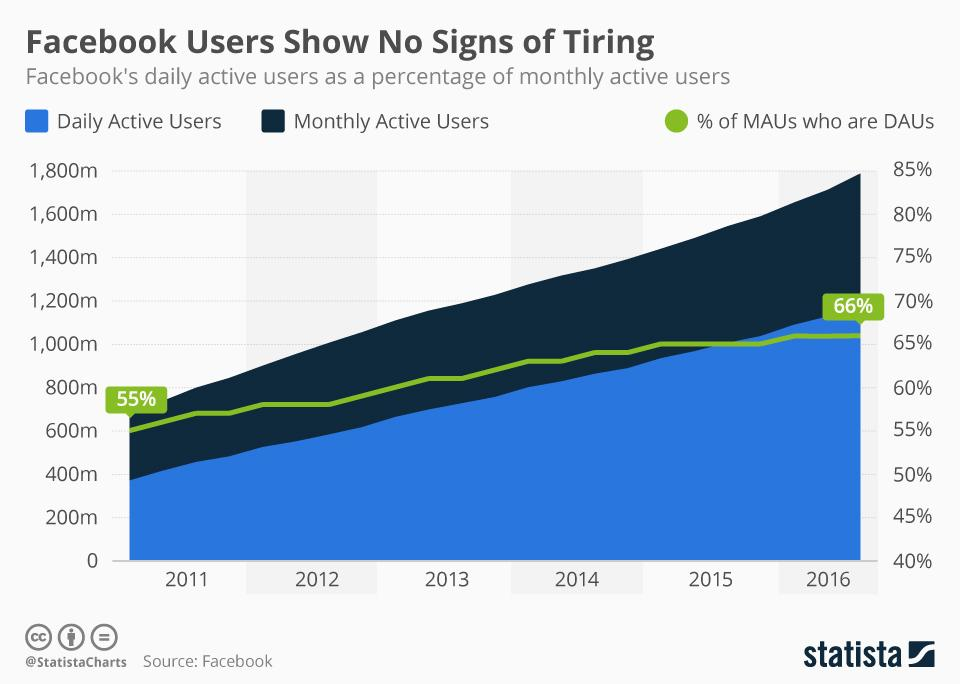
\includegraphics[width=15cm]{images/image5}
\centering
\caption[Figura 3.1]{Evolució de l’activitat diària i mensual dels usuaris de Facebook.}
\centering
\end{figure}

\subsection{Objectiu principal}

L’objectiu principal del projecte és la implementació d’una xarxa social adaptada a les persones amb diversitat funcional de dèficit cognitiu de grau mitja/baix.

\subsection{Objectius específics}

A part de l’objectiu principal del projecte, tenim uns quants objectius específics, els quals alguns d’aquest, ajuden a complir amb l’objectiu principal del projecte:

\begin{itemize}
	\item Disseny d’una interfície gràfica fàcilment manejable per persones amb baix nivell d’escriptura.
	\item Implementació d’una eina de gestió/monitoratge per a les associacions o professionals en l’àmbit.
	\item Dissenyar la xarxa social de forma que sigui responsive als diferents dispositius en els quals es podrà visitar.
	\item Implementar un sistema de seguretat, de forma que la gent que utilitzi la xarxa social siguin els usuaris amb diversitat funcional de dèficit cognitiu o professionals relacionats en l’àmbit.
	\item Implementar la xarxa de forma que accepti diferents idiomes.
\end{itemize}

\chapter{Gestió del Projecte}

\section{Abast}

L’abast del projecte vindrà donat per la implementació de dos elements essencials:

\begin{itemize}
	\item La implementació de la xarxa social per a persones amb diversitat funcional de dèficit cognitiu. Per satisfer aquest objectiu s’ha de pensar en les funcionalitats mínimes que ha de satisfer una xarxa social. Les funcionalitats mínimes que tindrà el sistema, seran les següents:
	\begin{itemize}
		\item L’usuari podrà publicar adreces d’interès, fotografies o simplement text (possiblement acompanyat d’iconografia) al seu mur.
		\item L’usuari es podrà fer amic dels altres usuaris per tal que aquests puguin veure les publicacions del seu mur.
		\item L’usuari podrà marcar “M’agrada” a les publicacions dels altres usuaris (sempre i quan siguin amics).
	\end{itemize}
	\item La implementació d’una eina de gestió per tal que els professionals de l’àmbit puguin gestionar i interactuar amb les persones que tracten en el món real. Les funcionalitats mínimes que tindrà el sistema són:
	\begin{itemize}
		\item Possibilitat d’invitar a persones amb diversitat funcional de dèficit cognitiu a entrar al sistema.
		\item Possibilitat de veure les publicacions de tots els usuaris que ha invitat.
	\end{itemize}
\end{itemize}

\subsection{Possibles obstacles}

Com en qualsevol projecte hi poden haver diversos obstacles, els quals poden dificultar el desenvolupament del software. Els obstacles possibles serien els següents:

\begin{itemize}
	\item \textbf{Temps limitat:} \\Aquest projecte té un temps bastant limitat, ja que té una data d’entrega fixa. Si no es té una bona organització del que s’ha de fer en cada moment, poden aparèixer imprevistos que puguin paralitzar el projecte. Per això, és necessari tindre una bona planificació, deixant un marge de temps per possibles imprevistos que puguin aparèixer.
	\item \textbf{Desconeixement de les tecnologies utilitzades:} \\Per desenvolupar el sistema s’utilitzaran tecnologies web i bases de dades no relacionals (Graph Database). Si aquestes no es coneixen prou, pot comportar que el desenvolupament del sistema sigui més lent i sense la qualitat suficient.
	\item \textbf{Accés a internet:} \\L’usuari del sistema necessitarà internet per poder fer-ne ús. Si aquest no té internet, aleshores no tindrà accés a la xarxa social i per tant no podrà interaccionar amb ningú mitjançant aquest sistema.
\end{itemize} 

\section{Metodología i rigor}

\subsection{Metodologies de treball} 

Per desenvolupar el projecte, s’utilitzarà scrum, el qual tractarà de definir diferents històries d’usuari (les quals representaran funcionalitats del sistema o necessitats del desenvolupador) amb uns certs punts d’història. Seguidament, es fixaran diferents dates en les quals, s’haurà d’haver acabat les històries d’usuari definides anteriorment (sempre per ordre de prioritat que el desenvolupador trobi oportú).\\ \\
Sí que és veritat que les metodologies àgils van molt encarades als treballs en grup, però considero que tot i ser un treball individual es poden aprofitar moltes idees per tal que el projecte aconsegueixi els seus objectius. Per exemple, el desenvolupament de cada funcionalitat amb completa independència de les altres.\\ \\
Les metodologies clàssiques (normalment en cascada), queden descartades, ja que el sistema que s’ha de desenvolupar tindrà moltes funcionalitats individuals, i la tecnologia en cascada, moltes vegades, implica fer canvis a les altres funcionalitats per tal d’aconseguir-ne una de nova.

\subsection{Eines de seguiment} 

En tractar-se d’un projecte software, considero que les eines de control de versions (Github i Bitbucked) són essencials. D’aquesta forma garantim que sempre tenim el codi disponible i que podem recuperar el codi anterior en cas que tinguem errors en les noves implementacions.


\subsection{Metodologies de treball} 

Per validar l’estat del projecte es passaran Unit Test, el qual tracta en testejar cadascuna de les funcionalitats del sistema un cop desenvolupades.\\ \\
A part, hi haurà vàries reunions amb el director per tal de garantir que el projecte segueix el camí establert inicialment.

\section{Planificació temporal}

\subsection{Planificació general}

\subsubsection{Durada estimada del projecte}

La durada estimada del projecte és de 6 mesos i mig, tenint en compte que el seu principi es troba en el moment en què vaig començar a fer recerca sobre el tema a tractar, principis de Desembre del 2016, i definint com a data final el dia de la defensa, que és a finals de Juny del 2017.

\subsubsection{Recursos}

Els recursos previstos per la realització d’aquest projecte són:

\begin{itemize}
	\item Recursos personals: Una persona, amb una dedicació al projecte de 25 hores setmanals.
	\item Recursos materials: Els recursos que s’utilitzaran en aquest projecte són els següents:
	\begin{itemize}
		\item \textbf{Control de versions:} Github o Bitbucked.
		\item \textbf{Servidor:} Perquè la pàgina estigui oberta les 24 hores del dia i els seus usuaris en puguin fer ús. A més, és on es trobarà la base de dades.
		\item \textbf{Correu Electrònic:} Per poder comunicar-me amb la gent que em faci falta per poder avançar el projecte.
		\item \textbf{WebStorm:} Framework de JetBrains per al desenvolupament Web.
		\item \textbf{Neo4j:} Base de dades no relacional (Graph Database), on es guardarà tota la informació dels usuaris.
		\item \textbf{GoogleDocs:} Eina d’edició de text que ens servirà per fer tota la documentació del projecte.
	\end{itemize}
\end{itemize}

\subsubsection{Pla d’acció i valoració d’alternatives}

La planificació del projecte es preveu flexible i modificable segons el ritme de desenvolupament del projecte.\\ \\
Es poden produir desviacions temporals en els diferents sprints o en el temps de dedicació a aprendre el funcionament d’una eina nova. Com que utilitzem una metodologia àgil, la qual implica crear sprints amb històries d’usuari (representen funcionalitats individuals del sistema i es mesuren en punts d’història), si una història no s’ha pogut acabar per un sprint, es ficarà pel següent. En el cas que els punts d’història que no s’han complert en un sprint siguin molt elevats, s’haurà de fer una replanificació del projecte, retallant alguna de les funcionalitats establertes a l’inici, per tal de tenir temps d’acabar-lo.\\ \\
Tot hi això, també es planificarà un sprint opcional, que ens servirà per desenvolupar funcionalitats extra en cas que les dates del projecte s’estiguin complint.

\subsubsection{Consideracions globals}

Encara que s'utilitzi una metodologia àgil, el projecte serà dut a terme per una sola persona, cosa que implica que no hi haurà desenvolupament de tasques en paral·lel. A més, es farà una llista de tasques, les quals és duran a terme seqüencialment, ordenades per prioritat del desenvolupador.\\ \\
Finalment, com que només hi haurà una persona que gestioni tot el projecte, el camí crític per satisfer totes les tasques és l’únic camí,  i per tant, trobem innecessari fer un diagrama de Pert.

\subsection{Descripció de les tasques}

\subsubsection{Posada en marxa}
En aquesta fase, l’autor farà recerca de la informació sobre el domini del projecte, necessària per al desenvolupament, i es prepararà l’entorn de treball. A més, es parlarà amb les parts interessades necessàries per resoldre els dubtes que es puguin ocasionar. Aquesta fase no té cap dependència de precedència.
	
\subsubsection{Gestió del Projecte (GEP)}
Aquesta fase consta de l’elaboració del document de gestió del projecte a partir de l’assignatura GEP. Aquesta fase no té cap dependència de precedència, però si que té un calendari estricte a seguir, ja que totes les entregues vénen donades en unes dates fixes.

\subsubsection{Desenvolupament de la xarxa social}
Elaboració de la primera part del producte, amb totes les fases del cicle de vida del desenvolupament d’un software incloses.  Aquesta tasca consistirà a desenvolupar tota la xarxa social, en la qual ja podrà ser usable pels usuaris. A més, es seguirà el següent seguit de fases: Planificació, Disseny, Implementació i Testeig. Les dependències de precedència d’aquesta etapa són les dues anteriors (Posada en marxa i Gestió del projecte).

\subsubsection{Desenvolupament de l’eina de gestió}
Elaboració de la segona part del producte, amb totes les fases del cicle de vida del desenvolupament d’un software incloses. Aquesta tasca consistirà a desenvolupar tota l’eina de gestió de la xarxa social, en la qual ja podrà ser usable pels professionals en l’àmbit. A més, es seguirà el següent seguit de fases: Planificació, Disseny, Implementació i Testeig. La dependència de precedència d’aquesta etapa és l’anterior (Desenvolupament de la xarxa social).

\subsubsection{Millores}
Opcional. Última tasca de desenvolupament del producte, on es contemplarà millores de funcionament o l’addició funcionalitats secundàries. Les dependències de precedència d’aquesta etapa són les dos anteriors (Desenvolupament de la xarxa social i Desenvolupament de l’eina de gestió).

\subsubsection{Documentació i Defensa}
Aquesta fase consistirà a acabar tota la documentació (memòria del projecte) i revisar que aquesta sigui correcta. La documentació s’anirà fent en les fases anteriors. A part, també es prepararà la defensa del projecte.\\ \\
La memòria del projecte inclourà tota la documentació redactada en el mòdul de GEP i la documentació derivada de les fases anteriors. El document final i la defensa tenen com a precedència totes les tasques anteriors del projecte.

\subsection{Calendari}

\subsubsection{Estimació d'hores}

\begin{table}[h]
\centering
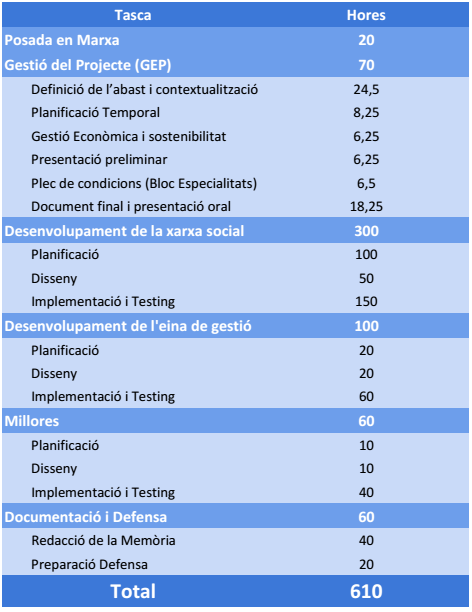
\includegraphics[width=12cm]{images/taula1}
\caption[Taula 6.1]{Estimació d'hores}
\centering
\end{table}

\newpage

\subsubsection{Diagrama de Gantt}

\begin{figure}[h]
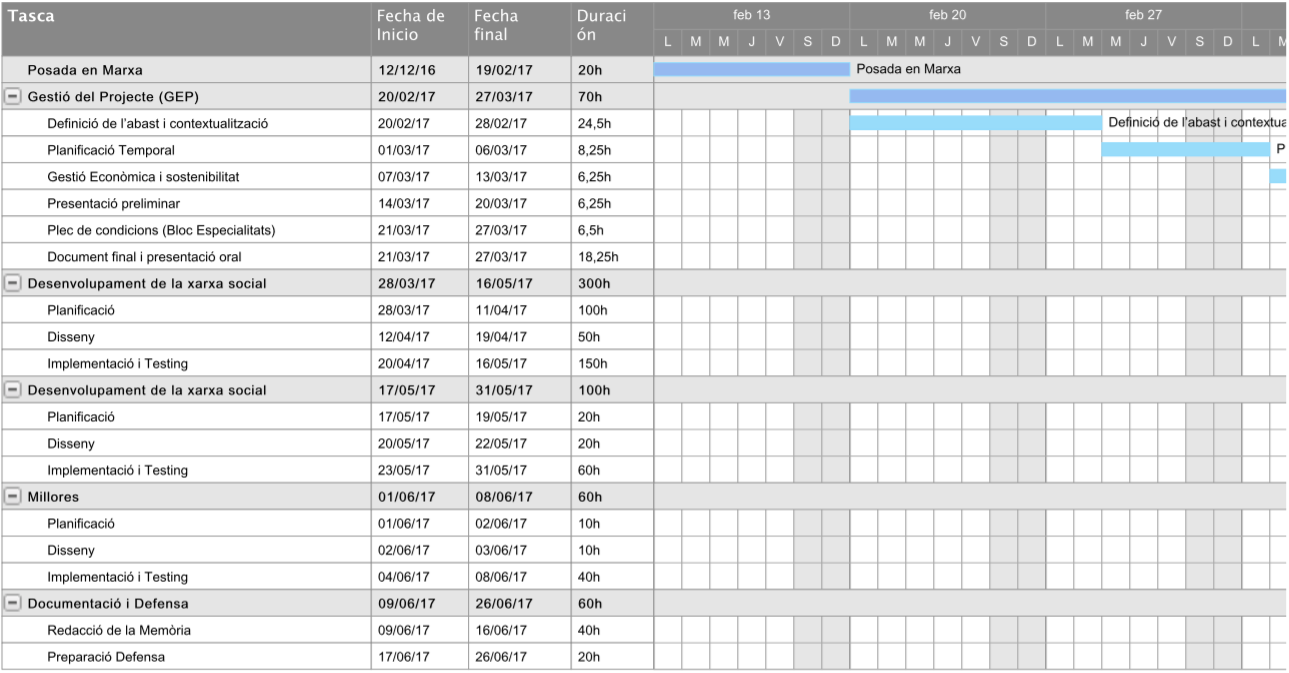
\includegraphics[width=14cm]{images/image2}
\centering
\end{figure}

\begin{figure}[h]
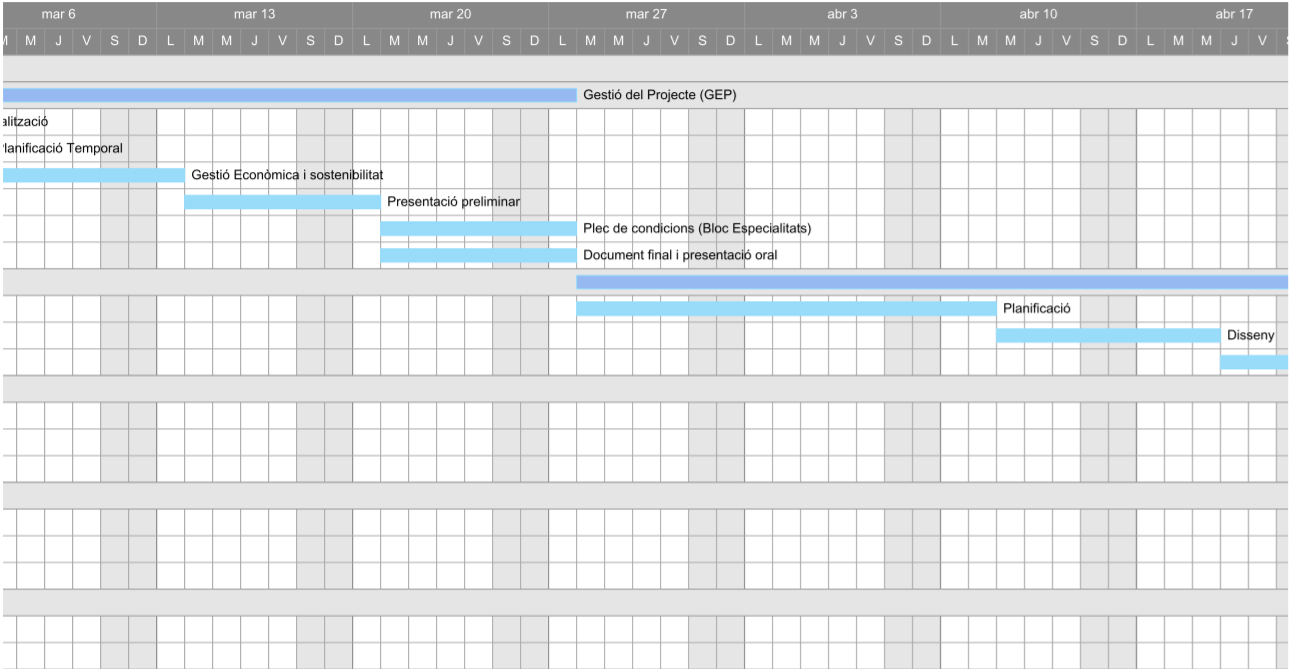
\includegraphics[width=14cm]{images/image8}
\centering
\end{figure}

\begin{figure}[h]
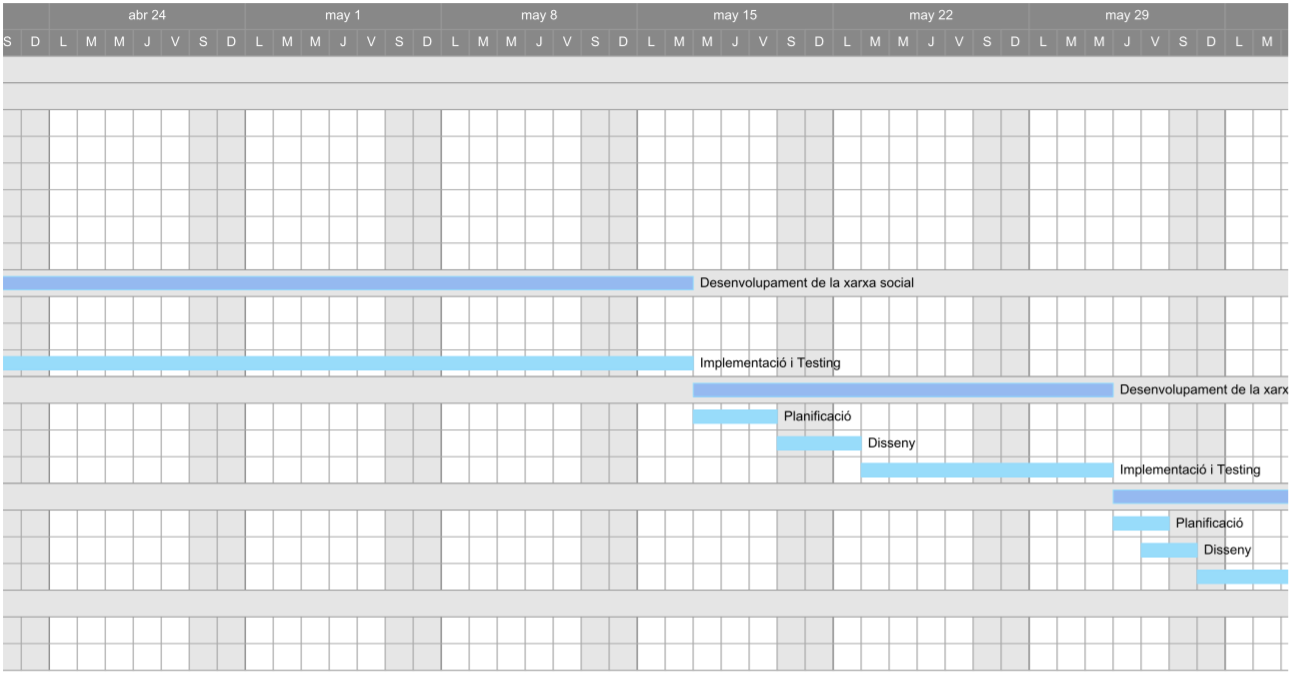
\includegraphics[width=14cm]{images/image4}
\centering
\end{figure}

\begin{figure}[h]
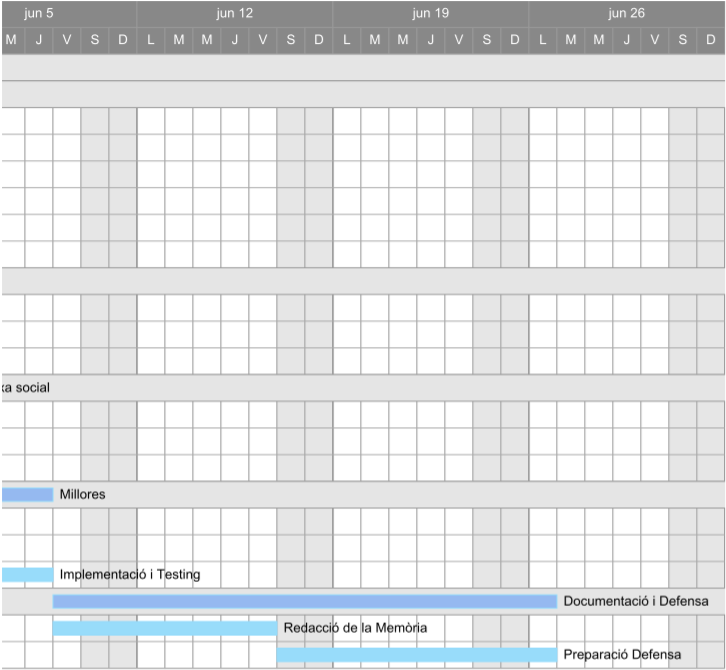
\includegraphics[width=14cm]{images/image7}
\centering
\caption[Figura 6.1]{Diagrama de Gantt}
\centering
\end{figure}

\clearpage
\section{Gestió Econòmica}

\subsection{Consideracions inicials}

En aquesta secció, identificarem tots els recursos necessaris per a la realització del projecte i farem una estimació del cost total d’aquests, tenint en compte aquestes dues variants:
\begin{itemize}
	\item Assumim que el projecte és universitari, i que per tant, no té una inversió econòmica.
	\item Assumim que és un projecte competitiu, amb les hores de recursos humans a preu de mercat.
\end{itemize}
A més, també s’explicarà com es durà a terme el control de la gestió durant tot el projecte.

\subsection{Identificació i estimació de costos}

\subsubsection{Costos directes}

Els costos directes per activitat en aquest projecte inclouen els recursos humans involucrats en cada una de les activitats definides al diagrama de Gantt presentat anteriorment. Encara que a la pràctica tot el projecte estigui desenvolupat per una sola persona, cada activitat d’aquest correspon a un rol diferent, i per tant, les hores tindran un preu de mercat diferent:

\begin{itemize}
	\item Tasques de gestió i documentació (Cap de Projecte): 50€/h.
	\item Anàlisis i disseny del producte (Analista): 40€/h.
	\item Implementació i proves (Programador): 35€/h.
\end{itemize}

A continuació trobem una taula amb el cost de mercat i el cost estimat d’aquest projecte:

\begin{table}[H]
\centering
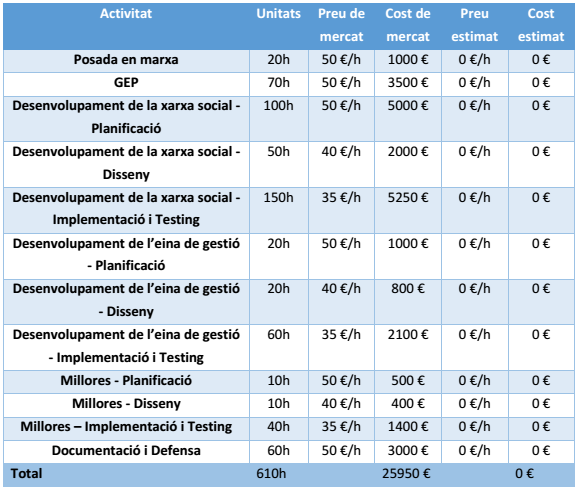
\includegraphics[width=11cm]{images/taula2}
\caption[Taula 7.1]{Costos directes}
\centering
\end{table}

\subsubsection{Costos indirectes}

En aquesta secció tindrem en compte tots els costos que ens afectin de forma indirecta, ho sigui, considerarem tots els costos que siguin necessaris pel projecte que siguin necessàries per a qualsevol projecte de software o que s’hagin de considerar en aquest projecte.
\begin{itemize}
	\item \textbf{Transport:} S’utilitzarà un abonament trimestral de 105 €. Com que l’abonament no depèn del nombre de viatges, considerarem que el cost extra és de 0%.
	\item \textbf{Software Extern:} S’intentarà fer servir software lliure i gratuït, de forma que el seu cost serà 0.
	\item \textbf{Impressions de paper:} el lliurament del projecte, inclou el lliurament de documentació. Suposarem que l’extensió de la memòria és d’unes 150 pàgines. Per altra banda, se’n han de fer 4 copies: 3 per als membres del tribunal i una pel director del projecte. Comptarem que cada pàgina costa uns 0,05 € (enquadernació inclosa).
	\item \textbf{Hardware:} L’únic hardware que s’utilitzarà en aquest projecte és un ordinador portàtil que ja es troba en ús. Suposant que la vida útil d’un portàtil és de 5 anys i que el 60\% del seu ús durant els propers 4 mesos estarà dedicat al projecte.
	\item \textbf{Connexió a internet:} Tot i que la connexió a internet és imprescindible per quasi qualsevol informàtic, considerarem que ja existeix una contractació. A partir d’aquí suposarem que de l’ample de banda consumit, se’n dedica un 20\% al projecte durant el temps que aquest duri.
\end{itemize} 

\begin{table}[h]
\centering
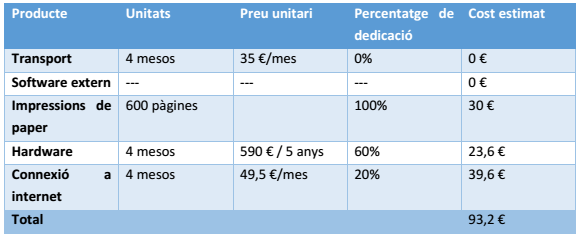
\includegraphics[width=15cm]{images/taula3}
\caption[Taula 7.2]{Costos indirectes}
\centering
\end{table}

\subsubsection{Contingència}

Per evitar qualsevol rics que hi pugui haver, reservarem una part del pressupost per a la part de contingència. Aquest cost serà un 15\% de la suma dels costos directes i indirecte.

\begin{table}[h]
\centering
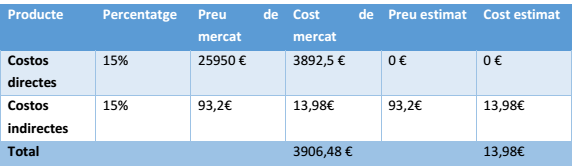
\includegraphics[width=15cm]{images/taula4}
\caption[Taula 7.3]{Contingència}
\centering
\end{table}

\subsubsection{Imprevistos}

Durant el projecte es poden presentar diferents imprevistos que ens facin encarir el projecte, els quals són:
\begin{itemize}
	\item \textbf{Avaria ordinador:} en cas que hi hagués algun problema amb el hardware, s’hauria de reparar o comprar-ne un de nou, augmentant el cost del projecte en màxim el preu de l’ordinador nou. Assignarem a aquesta eventualitat una probabilitat del 5\%.
	\item \textbf{Retard de 8 dies:} com que en la planificació temporal ja hem fet una reserva de millores del projecte, en cas de que aquest s’allargui s’utilitzarà aquesta reserva per acabar-lo.
\end{itemize}

\begin{table}[H]
\centering
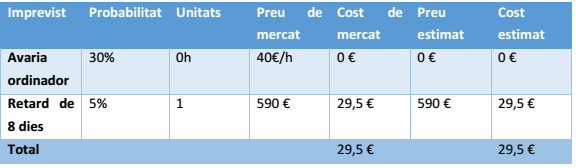
\includegraphics[width=15cm]{images/taula5}
\caption[Taula 7.4]{Imprevistos}
\centering
\end{table}

\subsubsection{Pressupost}

Durant el projecte no es consideren les següents situacions:
\begin{itemize}
	\item No es tenen en compte els augments de preu (escalació) durant el projecte, ja que es de curta durada i no es preveu que es doni la situació.
	\item No hi ha cap marge de benefici, ja que el projecte és completament sense ànim de lucre i no està destinat a la venda d’un producte.
\end{itemize}

\begin{table}[H]
\centering
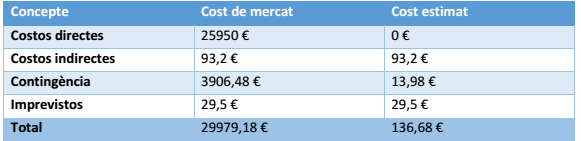
\includegraphics[width=15cm]{images/taula6}
\caption[Taula 7.5]{Pressupost}
\centering
\end{table}

\subsection{Control de gestió}

Per poder preveure les desviacions a nivell de temps, durant la realització del projecte, es mantindrà un registre d’hores amb data i concepte per tal de veure si es sobrepassa el número d’hores planificat. A més, a l’hora de fer cada una de les iteracions, com ja hem especificat a l’apartat de metodologia i rigor, és durà a terme amb metodologies àgils, cosa que ens donarà bastant marge de planificació en el cas que preveiem que s’hagi d’allargar el projecte, ja que les metodologies àgils ens donen l’opció de fragmentar molt les tasques en tasques més petites.\\ \\
Al final del projecte, quan ja es tinguin les hores reals que s’han dedicat al projecte i els costos indirectes, es farà una comparació amb la previsió inicial.\\ \\
En cas de que la comparativa sigui molt extrema es mirarà quines han sigut les causes que han provocat aquesta situació. Si el cost real ha sigut major al pressupostat, es mirarà si ha sigut degut als imprevistos que s’han tingut en compte i si es pot cobrir amb la partida corresponent. Si no es pot, s’assignarà la partida de contingència per cobrir-ho. Només es tindran en compte els costos indirectes, la partida d’imprevistos i la partida de contingència.

\section{Sostenibilitat i compromís social}

En aquest apartat, es farà una breu descripció de com afecta el projecte a nivell econòmic, social i ambiental.

\begin{table}[H]
\centering
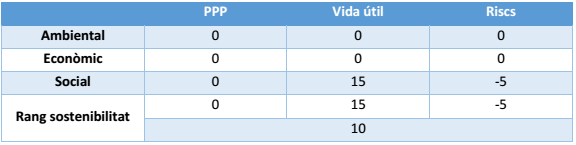
\includegraphics[width=15cm]{images/taula7}
\caption[Taula 7.5]{Pressupost}
\centering
\end{table}

\subsection{Econòmica}

Com que el projecte és sense ànim de lucre, he decidit punta’l en 0 punts a nivell econòmic. Ja que no està pensat per fer-hi negoci, sinó a ser una eina que ajudi a integrar a la societat totes aquelles persones que ho necessiten i no tenen l’oportunitat de fer-ho.

\subsection{Social}

L’objectiu principal del projecte, és donar l’opció de poder utilitzar una xarxa social a persones amb diversitat funcional de dèficit cognitiu amb unes nocions mínimes de lectura i escriptura. Per tant, com que el projecte està encarat a fer una ajuda social, he decidit ficar-li 15 punts d’impacte social. \\ \\
També existeix algun risc social en aquest projecte, ja que pot haver-hi persones que el categoritzin de marginació social pel fet de que només i tinguin accés persones amb diversitat funcional de dèficit cognitiu, o professionals relacionats en l’àmbit. Per això, he decidit ficar-li -5 punts de risc social.

\subsection{Ambiental}

He decidit puntuar tota la secció ambiental amb 0 punts, ja que el projecte no ajuda ni perjudica el medi ambient. A més no és preveu la dependència de cap recurs en acabar el projecte, ni necessitarem cap producte nou.


\chapter{Seguiment del Projecte}

\section{Introducció}

En aquest capítol, es definirà quin ha sigut el seguiment del projecte i com s'ha dut a terme. \\ \\
Ja que en el projecte s'utilitzen les metodologies àgils, s'ha definit un product backlog inicial amb totes les històries a realitzar durant el projecte. A més, la planificació temporal s'ha dividit en 6 sprints:
\begin{itemize}
\item 3 Sprints pertinents al desenvolupament de la xarxa social.
\item 2 Sprints pertinents al desenvolupament de l'eina de gestió.
\item 1 Sprint pertinent a la part de millores.
\end{itemize}
Abans de realitzar cada un dels sprints, es seleccionen les històries del backlog que es realitzaran. Quan aquest finalitza, les històries que no s'han acabat es retornen al backlog, o en casos molt específics, es descarten del projecte.\\ \\
En aquesta secció es descriurà quin ha sigut el backlog inicial, i com s'ha procedit en cada un dels sprints. Cada un dels sprints estarà definit pels següents apartats: Resum de l'sprint, Descripció i resultat de les històries d'usuari, tecnologies utilitzades (només en els casos en què s'en afegeixi alguna) i conclusions de l'sprint.
\newpage
\section{Product Backlog}

El product backlog inicial del projecte ha sigut el següent:

\begin{table}[H]
\centering
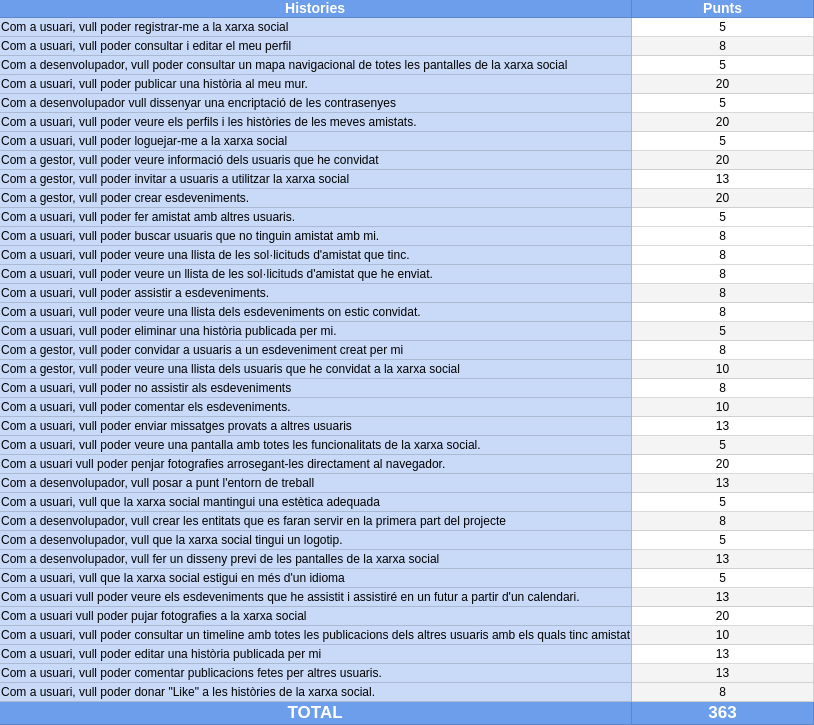
\includegraphics[width=15cm]{images/taula8}
\caption[Taula 7.5]{Product Backlog}
\centering
\end{table}

\section{Sprint 1}

\subsection{Resum de l'sprint}

L'sprint no ha anat dins dels marges esperats. Dels 64 punts definits en aquest sprint, només se n'han aconseguit 31.\\ \\
Això es deu al poc coneixement de les tecnologies que s'havien d'utilitzar a priori, i que per tant s'ha fet molt difícil a l'hora d'utilitzar-les. També cal dir que moltes d'aquestes tecnologies s'han hagut de buscar en el moment que ha sortit la necessitat d'utilitzar-les i s'han convertit en requisits emergents dins del projecte.\\ \\
En els apartats següents veurem quines són les tasques que s'han dut a terme en aquest sprint i quin ha sigut el seu resultat.

\subsection{Descripció i resultat de les històries d'usuari}

\subsubsection{Com a desenvolupador, vull posar a punt l'entorn de treball (13 punts)}

Aquesta història ha consistit a buscar i instal·lar totes les tecnologies necessàries per posar en marxa el projecte. S'ha dividit en les següents tasques:
\begin{itemize}
\item Instal·lar IntellIJ Webstorm.
\item Instal·lar Node.js.
\item Buscar servei de núvol on puguem penjar la pàgina web.
\item Instal·lar els paquets necessaris de Node.js.
\item Creació del repositori de GitHub.
\end{itemize}
\textcolor{forestgreen}{\textbf{Resultat:}} Totes les tasques que s'han descrit en aquesta història s'han completat en el temps estimat. El problema ha vingut a l'hora de començar a implementar la història "Com a usuari, vull poder registrar-me a la xarxa social" de l'sprint (la qual veurem més endavant), ja que hi ha hagut molts requisits emergents que no s'han tingut en compte anteriorment, i per tant, el temps d'aquesta història ha augmentat moltíssim.

\subsubsection{Com a usuari, vull que la xarxa social mantingui una estètica adequada (5 punts)}

Aquesta història ha consistit a buscar els colors o fonts (tipus de lletra) perquè la pàgina web tingui una estètica agradable a la vista de l'usuari. S'ha dividit en les següents tasques:
\begin{itemize}
\item Buscar els colors primaris.
\item Buscar una font.
\end{itemize}
\textcolor{forestgreen}{\textbf{Resultat:}} No ha sigut molt difícil trobar els colors primaris i les fonts principals de l'aplicació. Els colors primaris són els següents:

\begin{figure}[h]

\includegraphics[width=12cm]{images/image1}
\centering
\caption[]{Paleta de colors de l'aplicació.}
\centering
\end{figure}

Per troba'ls, he utilitzat una eina que es diu \textbf{paletton}, la qual et permet combinar colors de forma senzilla. Per utilitzar-la podeu entrar a la següent URL: \\ \\
\url{http://paletton.com/\#uid=5300u0kqALsd8VjkyQ8B3GbBuoR} \\ \\
L'aplicació estarà composta per dues fonts:
\begin{itemize}
\item \textbf{Montserrat:} És la font que s'utilitzarà en els títols.
\item \textbf{Raleway:} S'utilitzarà per a la resta de text de l'aplicació.
\end{itemize}

\subsubsection{Com a desenvolupador, vull crear les entitats que es faran servir en la primera part del projecte (8 punts)}

Aquesta història ha consistit a crear les entitats de dades que guardarem a la base de dades. S'ha dividit en les següents tasques:
\begin{itemize}
\item Creació de l'entitat 'Usuari'
\item Creació de l'entitat 'Història'
\item Creació de l'entitat 'Esdeveniment'
\end{itemize}
\textcolor{forestgreen}{\textbf{Resultat:}} Aquesta història va tenir una molt mala estimació de cost, ja que el temps en què s'ha realitzat ha sigut bastant ràpid. Les entitats resultants són les següents:

\begin{figure}[h]
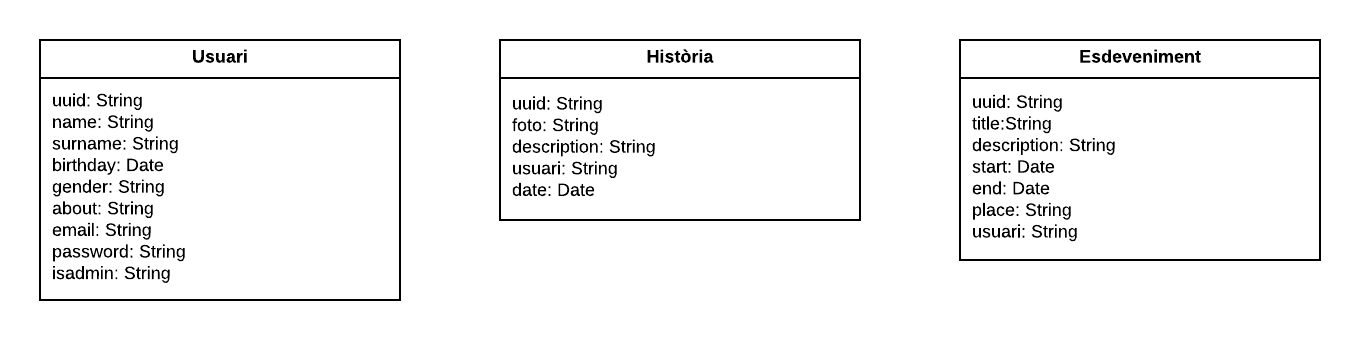
\includegraphics[width=15cm]{images/image6}
\centering
\caption[]{Entitats de l'aplicació.}
\centering
\end{figure}

\subsubsection{Com a desenvolupador, vull que la xarxa social tingui un logotip (5 punts)}

Aquesta història ha consistit en la creació d'un logotip per utilitzar en la nostra aplicació web. S'ha dividit en les següents tasques:
\begin{itemize}
\item Buscar Imatges pel logotip.
\item Creació del logotip.
\end{itemize}
\textcolor{forestgreen}{\textbf{Resultat:}} La tasca s'ha realitzat correctament, i dins de l'estimació donada en punts. Per fer el logotip de l'aplicació, s'han utilitzat les mateixes fonts que s'han triat en la història "Com a usuari, vull que la xarxa social mantingui una estètica adequada" d'aquest sprint.
El resultat és el següent:

\begin{figure}[H]

\includegraphics[width=7cm]{images/image3}
\centering
\caption[]{Logotip de l'aplicació.}
\centering
\end{figure}

\subsubsection{Com a desenvolupador, vull poder consultar un mapa navigacional de totes les pantalles de la xarxa social (5 punts)}

\textcolor{costumyellow}{\textbf{Resultat:}} Com hem vist anteriorment, la història "Com a desenvolupador, vull posar a punt l'entorn de treball" d'aquest sprint ens ha fet perdre molt temps. Temps que s'hagués pogut invertir a fer la resta d'històries. Per tant, al veure que no necessitàvem un mapa navigacional en aquest sprint, he decidit deixar aquesta història per l'sprint 2.

\subsubsection{Com a desenvolupador, vull fer un disseny previ de les pantalles de la xarxa social (13 punts)}

\textcolor{red}{\textbf{Resultat:}} Durant l'sprint, a l'hora de ficar-me a fer aquesta història, em vaig adonar que el cost d'aquesta era molt elevat, i que per tant era una pèrdua de temps fer aquest disseny. Comptant que el temps per fer el projecte és molt poc i que el seu valor no és molt elevat pel projecte, he decidit retirar aquesta història.

\subsubsection{Com a usuari, vull que la xarxa social estigui en més d'un idioma (5 punts)}

\textcolor{red}{\textbf{Resultat:}} Vaig estar buscant alguna forma de simplificar l'aplicació i ficar els literals (paraules fixes que es troben a l'aplicació) en un mateix fitxer. La solució que vaig trobar era bastant difícil d'implementar i feia pujar els punts d'aquesta història. Per consegüent, he optat que per cada pàgina de l'aplicació, hi haurà 3 versions (una en anglès, una en castellà i una altra en català). Per tant, la història es retira del backlog inicial.

\subsubsection{Com a usuari, vull poder registrar-me a la xarxa social (5 punts)}

\textcolor{costumyellow}{\textbf{Resultat:}} La història "Com a desenvolupador, vull posar a punt l'entorn de treball" ens ha tret molt de temps d'aquest sprint, i conseqüentment, aquesta història no s'ha pogut acabar i queda per l'sprint 2.

\subsubsection{Com a usuari, vull poder loguejar-me a la xarxa social (5 punts)}

\textcolor{costumyellow}{\textbf{Resultat:}} La història "Com a desenvolupador, vull posar a punt l'entorn de treball" ens ha tret molt de temps d'aquest sprint, i conseqüentment, aquesta història no s'ha pogut ni començar i queda per l'sprint 2.

\subsection{Tecnologies utilitzades}

\subsubsection{Tecnologies Web}

Aquesta tecnologia és necessària per al funcionament de l'aplicació. Si l'aplicació no es troba en el núvol, aquesta no és accessible pels usuaris, i per tant perd el seu valor. \\ \\
La tecnologia que he triat per utilitzar es diu Heroku (\url{https://www.heroku.com}), i és una plataforma d'aplicacions al núvol. Aquesta plataforma permet tindre la teva pàgina web en línia les 24h, i a més, té un sistema de storage, on es guarden totes les dades generades pels usuaris de la pàgina.\\ \\
La URL a la pàgina on es troba l'aplicació d'aquest projecte és: \\
\url{https://makeyourfriend.herokuapp.com}

\subsubsection{IDE}

Com que el projecte és web, també s'ha d'utilitzar una IDE encarada a aquest propòsit. La que he triat per aquest projecte es diu IntellIJ WebStorm (\url{https://www.jetbrains.com/webstorm}), i és una IDE que està encarada al Javascript, però que també accepta tot el que vindria a ser els llenguatges de frontend, com HTML o CSS.\\ \\
La llicència d'aquesta IDE, és de pagament, però al ser estudiant de la FIB et surt gratuïta.

\subsubsection{Bases de Dades}

Com que l'aplicació és una xarxa social, una base de dades relacional no és tan eficient, ja que sempre ha d'estar buscant a les taules. Per consegüent, he decidit utilitzar una base de dades no relacional anomenada neo4j (\url{https://neo4j.com}). Aquesta base de dades és una graph database que permet crear nodes (on es guarda la informació de l'usuari, històries o esdeveniments) i seguidament relacionar-los entre ells amb una etiqueta. \\ \\
La seva eficiència en aquest tipus d'aplicacions, cau en què no cal que tinguem una taula amb totes les amistats. Si volem saber quines amistats té un usuari, ens fiquem al node d'aquest usuari i mirem les arestes que contenen el tag "Amistat". Aquestes arestes ens porten directament als nodes de les amistats.\\ \\
Finalment, ni que en aquest sprint no s'hagi fet, segurament serà necessari una base de dades relacional per emmagatzemar les fotografies de l'aplicació i guanyar eficiència. Quan una fotografia es guarda en una base de dades, s'encripta amb un string (que ocupa molt espai), i per tant, costaria molt fer una cerca per la base de dades.

\subsubsection{Framework}

El framework utilitzat pel projecte és Node.js (\url{https://nodejs.org}). És un framework que et facilita totes les feines encarades a web. Els seus llenguatges bàsics són HTML, CSS i Javascript, tot i que pots afegir les funcionalitats que vulguis instal·lant els paquets necessaris al teu projecte.\\ \\
Finalment, dir que aquest framework et dóna molta facilitat per implementar la comunicació client servidor.

\subsubsection{Paquets addicionals de Node.js}

Com he dit a l'apartat anterior, Node.js et permet instal·lar paquets amb funcionalitats extra al teu projecte. Els paquets que s'ha utilitzat en aquest sprints són els següents:
\begin{itemize}
\item \textbf{body-parser:} Aquest paquet ens permet llegir els camps que ha omplert el client directament des del servidor, sense la necessitat d'haver de fer una crida ajax per passar els paràmetres.
\item \textbf{bootstrap:} És un framework per HTML, CSS i Javascript que permet fer les pàgines responsive amb facilitat.
\item \textbf{dotenv:} ens permet carregar fitxers .env a l'aplicació.
\item \textbf{jquery:} És una llibreria de Javascript que et permet escriure el mateix codi de forma més ràpida, i que permet la manipulació del codi HTML de forma senzilla.
\item \textbf{jquery-validation:} És un pluguin de jQuery que serveix per validar els diferents formularis que hi puguin haver a l'aplicació (dates, correus electrònics, contrasenyes, etc).
\item \textbf{neo4j-driver:} És un driver que permet configurar connexions amb Neo4j, ja explicat a l'apartat 3.3.
uuid: Ens permet auto generar un identificador únic per a cada node de la base de dades.
\item \textbf{pug:} Aquest paquet permet escriure el codi HTML més ràpidament i permet crear bucles d'informació dinàmica a la pàgina web.
\item \textbf{font-awesome:} És una llibreria d'icones.
\item \textbf{w3-css:} Permet fer dissenys més amistosos per l'usuari de l'aplicació amb facilitat.

\end{itemize}

\subsection{Conclusions de l'sprint}

Com podem veure, durant aquest sprint s'han fet menys de la meitat dels punts que estaven previstos. Tot hi això, ja tenim quasi totes les tecnologies necessàries instal·lades a l'aplicació i per tant, serà més fàcil utilitzar-les.\\ \\
Sí que és possible que durant l'sprint 2 sorgeixi la necessitat d'alguna tecnologia més, però preveig que seran molt poques.


\section{Sprint 2}

\subsection{Resum de l'sprint}

L'sprint a complert amb els requisits establerts inicialment. Dels 73 punts definits en aquest sprint, s'han complert tots.\\ \\
Com s'ha comentat en l'sprint anterior, ficar a punt l'entorn de treball, em va treure molt temps del qual s'havia establert inicialment. Com que l'entorn ja es va ficar a punt en l'sprint anterior, en aquest sprint no hem tingut el mateix problema, i per tant s'ha pogut complir amb tots els requeriments.\\ \\
En els apartats següents veurem quines són les tasques que s'han dut a terme en aquest sprint i quin ha sigut el seu resultat. També es veuran quines han sigut les tecnologies que s'han incorporat al projecte.

\subsection{Descripció i resultat de les històries d'usuari}

\subsubsection{Com a usuari, vull poder registrar-me a la xarxa social (5 punts)}

Aquesta història ha consistit en la implementació d'una pàgina de registre per la xarxa social. La pàgina de registre conté els següents camps:
\begin{itemize}
\item \textbf{Nom:} El camp contindrà el nom de l'usuari (o el nom amb el qual vulgui ser reconegut pel sistema).
\item \textbf{Cognoms:} El camp contindrà els cognoms de l'usuari.
\item \textbf{Gènere:} En aquest camp s'indicarà si l'usuari és un home o una dona.
\item \textbf{Data de naixement:} En aquest camp s'informarà la data de naixement de l'usuari.
\item \textbf{Correu Electrònic:} En aquest camp s'informarà el correu electrònic de l'usuari, el qual servirà com identificador del sistema.
\item \textbf{Sobre tu:} En aquest camp es pot afegir una breu descripció sobre el mateix usuari.
\item \textbf{Contrasenya:} El camp es repeteix dues vegades (per assegurar que te'n recordaràs de la contrasenya). La contrasenya haurà de tindre un mínim de 8 caràcters perquè sigui vàlida.
\item \textbf{Codi d'invitació:} En aquest camp s'haurà d'informar el codi que l'administrador haurà informat amb anterioritat a l'usuari.
\end{itemize}
\textcolor{forestgreen}{\textbf{Resultat:}} La història s'ha realitzat amb èxit, tot i que el seu cost estava una mica mal estimat. En veritat ha portat més dels 5 punts estimats inicialment.

\subsubsection{Com a usuari, vull poder loguejar-me a la xarxa social (5 punts)}

La història ha consistit a poder fer login a l'aplicació informant el correu electrònic i la contrasenya registrats en l'història anterior.\\ \\
\textcolor{forestgreen}{\textbf{Resultat:}} La història no ha portat cap problema i s'ha realitzat amb el cost estimat.

\subsubsection{Com a desenvolupador vull dissenyar una encriptació de les contrasenyes (5 punts)}

Aquesta història s'ha dividit en dues tasques:
\begin{itemize}
\item Encriptació de la contrasenya.
\item Manutenció de les sessions dels usuaris.
\end{itemize}
\textcolor{forestgreen}{\textbf{Resultat:}} La primera tasca de la història s'ha utilitzat la llibreria crypto de Node.js, la qual et permet encriptar una contrasenya en base64 utilitzant l'algoritme "sha256". En la segona tasca s'ha utilitzat la llibreria client-session de Node.js, la qual permet mantenir sessions mitjançant les cookies del navegador utilitzat. Els punts de la història s'han estimat adequadament.

\subsubsection{Com a usuari, vull poder consultar i editar el meu perfil (8 punts)}

La història s'ha dividit en dues parts:
\begin{itemize}
\item Oferir l'oportunitat de poder consultar el teu propi perfil.
\item Poder editar el teu propi perfil. Aquesta tasca s'ha dividit en dos més:
\begin{itemize}
\item Poder canviar la teva foto de perfil (o ficar-ne una en cas que no en tinguis).
\item Poder canviar la descripció del teu usuari (el camp "Sobre tu" que s'informa en el registre d'un usuari).
\end{itemize}
\end{itemize}
\textcolor{forestgreen}{\textbf{Resultat:}} Els punts de la història s'han estimat correctament, i s'ha aconseguit tot el que es demanava. S'ha de dir, que la part de canviar la fotografia de perfil s'ha dut a terme en la història "Com a usuari vull poder pujar fotografies a la xarxa social" la qual es veurà més endavant.

\subsubsection{Com a usuari, vull poder veure una pantalla amb totes les funcionalitats de la xarxa social (5 punts)}

Aquesta història ha consistit en crear una pantalla on l'usuari pogués veure amb facilitat totes les funcions de la xarxa social. Les diferents funcions que té són: El meu perfil, les meves històries, els meus amics, els meus esdeveniments, línia temporal, buscar amics, publicar història.\\ \\
\textcolor{forestgreen}{\textbf{Resultat:}} La història s'ha estimat de forma adequada i s'ha dut a terme correctament.

\subsubsection{Com a desenvolupador, vull poder consultar un mapa navigacional de totes les pantalles de la xarxa social (5 punts)}

La història ha consistit en crear un mapa navigacional de les pantalles que pot utilitzar l'usuari del sistema (amb usuari ens referim al fet que no és un administrador de la xarxa), utilitzant nomenclatura UML.\\ \\
\textcolor{forestgreen}{\textbf{Resultat:}} La història s'ha estimat de forma adequada i s'ha dut a terme correctament. El resultat és el següent:

\begin{figure}[H]
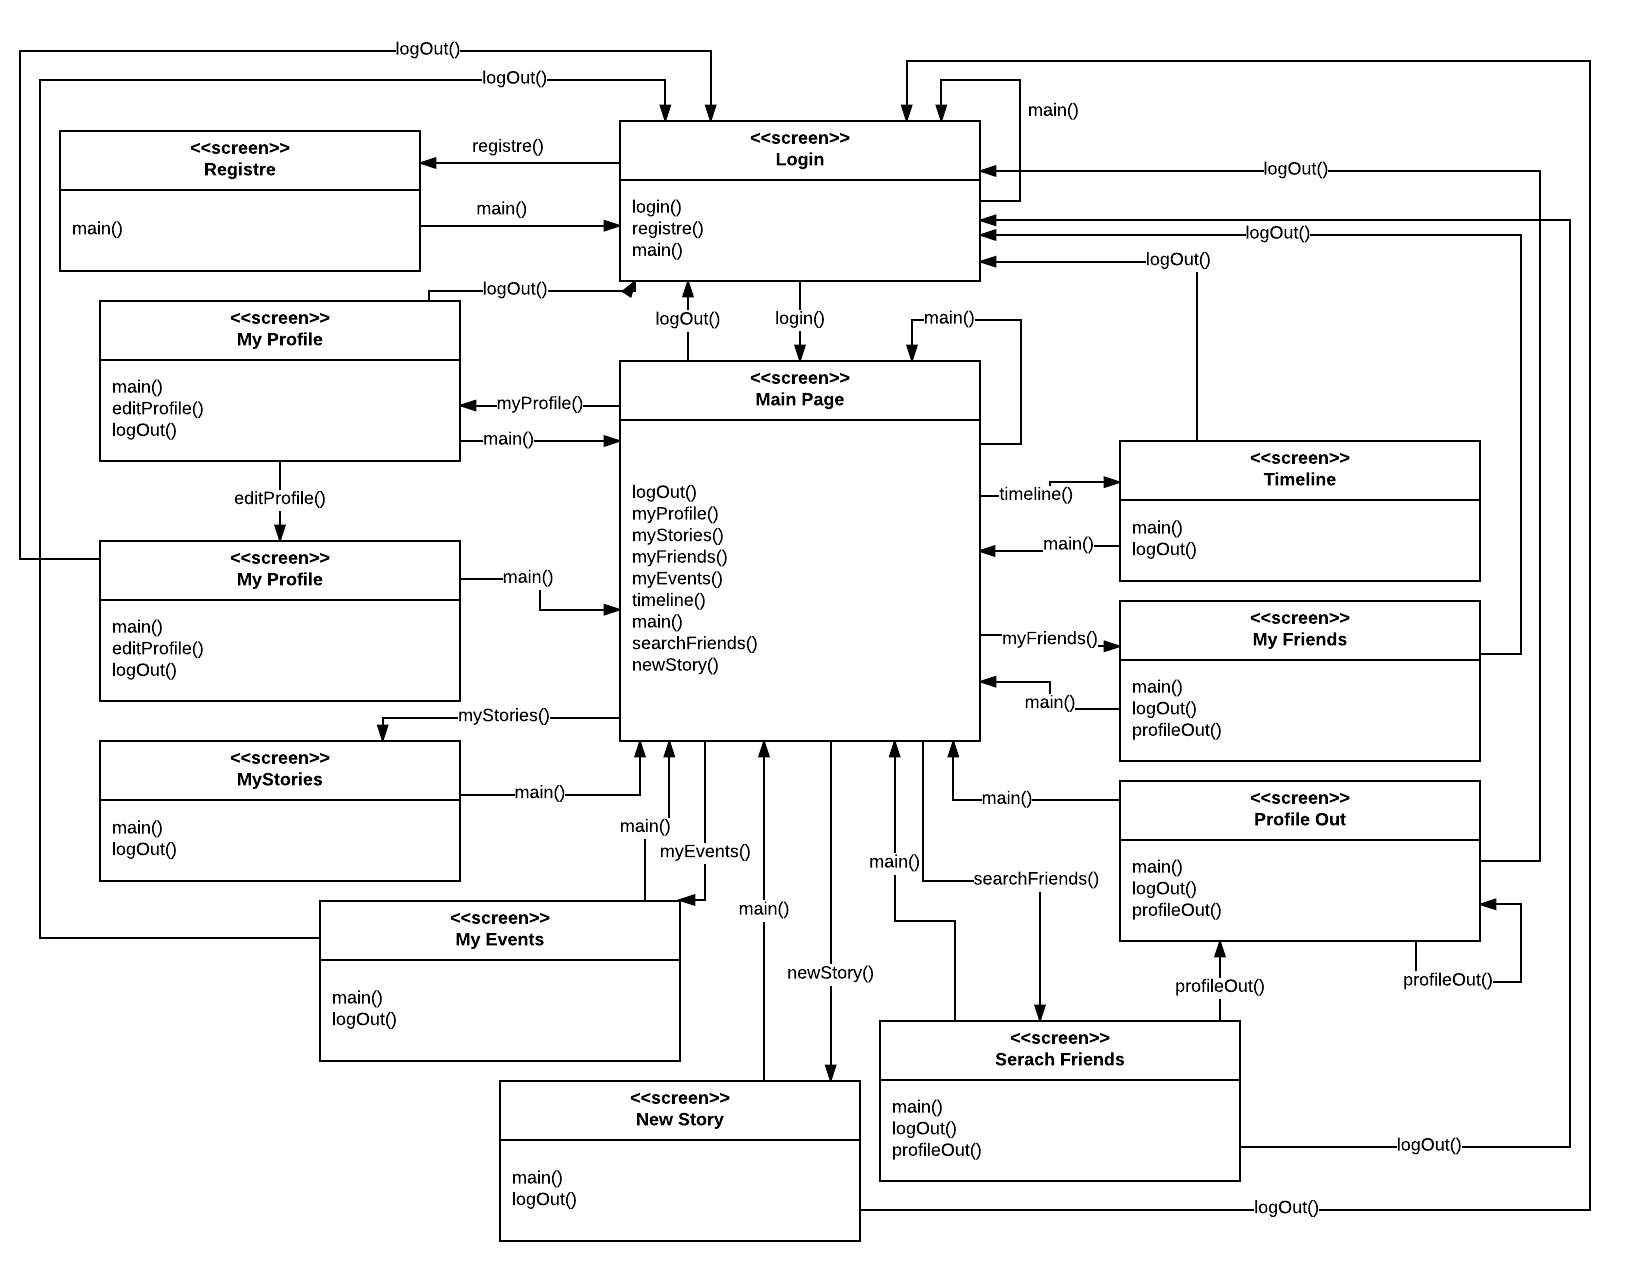
\includegraphics[width=15cm]{images/image9}
\centering
\caption[]{Mapa navigacional de l'aplicació (Només usuari).}
\centering
\end{figure}
Com bé podem veure, en aquest mapa navigacional, es pot observar quines seran les diferents pantalles del sistema i com arribar a cada una d'elles. Remarcar, que aquestes pantalles només representen les pantalles accessibles pels usuaris, ja que un administrador tindrà la funcionalitat de poder crear esdeveniments.

\subsubsection{Com a usuari, vull poder publicar una història al meu mur (20 punts)}

La història ha consistit en donar l'oportunitat a l'usuari per poder publicar històries al seu mur. Per poder fer-ho, s'ha hagut de emplenar un formulari amb els següents camps:
\begin{itemize}
\item \textbf{Imatge o fotografia:} Et permet penjar una fotografia a la història.
\item \textbf{Descripció:} Permet afegir una descripció a la història.
\end{itemize}
\textcolor{forestgreen}{\textbf{Resultat:}} S'ha dut a terme correctament i s'ha estimat adequadament. Igual que la història anterior, la part de penjar la fotografia s'ha dit a terme en la història "Com a usuari vull poder pujar fotografies a la xarxa social".

\subsubsection{Com a usuari vull poder pujar fotografies a la xarxa social (5 punts)}

La història ha consistit en poder pujar fotografies a la xarxa social, tant al teu perfil com a les històries que es vulguin publicar.\\ \\
\textcolor{forestgreen}{\textbf{Resultat:}} La tasca s'ha dut a terme correctament, tot i que el temps que s'ha utilitzat per completar-la s'ha allargat més del que s'havia previst. Per poder pujar fotografies a la xarxa social he agut d'utilitzar una llibreria de Node.js anomenada multer, la qual et permet pujar fotografies de forma senzilla.\\ \\
Inicialment, volia fer que es pengessin les fotografies utilitzant un drag \& drop des de l'escriptori de l'ordinador fins a la pàgina web. Per fer-ho he trobat moltes complicacions, cosa que ha comportat la creació d'una nova història: "Com a usuari vull poder penjar fotografies arrossegant-les directament al navegador".

\subsection{Tecnologies utilitzades}

\subsubsection{Bases de Dades}

En l'sprint anterior, s'havia comentat de què les fotografies s'emmagatzemarien utilitzant una base de dades SQL, tot i que això al final no ha sigut possible.\\ \\
He estat intentant que en el moment que la imatge arribés al servidor, aquesta es guardés a la base de dades SQL (postgres), però no hi ha hagut manera d'aconseguir-ho, i per tant les imatges es guarden en una jerarquia de directoris al mateix servidor.\\ \\
Les fotografies de perfil es guardaran en el directori "uploadsProfile" i les imatges de les històries es guardaran en el directori "uploadsPost". Una vegada les imatges estiguin guardades en el directori corresponent, s'actualitzaran els camps foto de les entitats Usuari i Història esmentades en l'sprint anterior.

\subsubsection{Paquets addicionals de Node.js}

En aquest sprint s'han utilitzat els següents paquets addicionals de Node.js:
\begin{itemize}
\item \textbf{crypto:} Aquest paquet ens permet encriptar les contrasenyes dels usuaris, en base64, utilitzant diferents algoritmes.
\item \textbf{client-session:} Paquet que ens permetrà mantenir les sessions dels usuaris.
\item \textbf{multer:} Paquet que permet al client penjar fotografies al servidor utilitzant funcions middleware.
\end{itemize}

\subsection{Conclusions de l'sprint}

Aquest sprint s'ha finalitzat correctament i dins del període establert, tot i que també n'ha sortit una nova història, la qual es durà a terme en l'sprint 3.

\section{Sprint 3}

\subsection{Resum de l'sprint}

Durant aquest sprint, s'han complert 64 dels 84 punts establerts inicialment, i es pot dir que la primera part del software (implementació de la xarxa social) s'ha acabat d'implementar.\\ \\
En els apartats següents veurem quines són les tasques que s'han dut a terme en aquest sprint i quin ha sigut el seu resultat. També es veuran quines han sigut les tecnologies que s'han incorporat al projecte.

\subsection{Descripció i resultat de les històries d'usuari}

\subsubsection{Com a usuari, vull poder buscar usuaris que no tinguin amistat amb mi (8 punts)}

La història ha consistit en poder buscar els usuaris que no tenen amistat amb mi. Aquesta cerca es podia fer de dues formes:
\begin{itemize}
\item Buscar tots els usuaris del sistema.
\item Buscar a partir d'una cadena de caràcters (els quals coincidissin amb part del nom o cognom de l'usuari).
\end{itemize}
\textcolor{forestgreen}{\textbf{Resultat:}} La història s'ha completat amb èxit.

\subsubsection{Com a usuari, vull poder veure un llista de les sol·licituds d'amistat que he enviat (8 punts)}
Aquesta història permet a l'usuari poder visualitzar una llista de les sol·licituds d'amistat que té pendents.\\ \\
\textcolor{forestgreen}{\textbf{Resultat:}} La història s'ha completat amb èxit.

\subsubsection{Com a usuari, vull poder veure una llista de les sol·licituds d'amistat que tinc (8 punts)}
Aquesta història permet a l'usuari poder visualitzar una llista de les sol·licituds d'amistat que aquest ha enviat a altres usuaris.\\ \\
\textcolor{forestgreen}{\textbf{Resultat:}} La història s'ha completat amb èxit.

\subsubsection{Com a usuari, vull poder fer amistat amb altres usuaris (5 punts)}
La història s'ha centrat en permetre crear amistat amb els usuaris utilitzant part de les històries anteriors que s'han dut a terme en aquest sprint.\\ \\
\textcolor{forestgreen}{\textbf{Resultat:}} La història s'ha completat amb èxit. Per fer-ho, s'han utilitzat dos tipus de relació entre els usuaris (que es representen en nodes a la base de dades):
\begin{itemize}
\item \textbf{MY\_REQUEST:} Relació d'un usuari cap a un altre que representa que un usuari ha enviat una sol·licitud d'amistat.
\item \textbf{MY\_FRIEND:} Una vegada l'amistat accepta la sol·licitud d'amistat, la relació anterior s'elimina de la base de dades, i seguidament, es creen dues relacions "MY\_FRIEND" entre els dos usuaris de la base de dades. Aquestes dues relacions es creen perquè en una graph database no es permet la creació de relacions bidireccionals.
\end{itemize}

\subsubsection{Com a usuari, vull poder veure els perfils i les històries de les meves amistats (20 punts)}

Aquesta història ha constat de dues parts:
\begin{itemize}
\item Poder visualitzar una llista amb totes les amistats de l'usuari.
\item Poder veure els perfils i les històries de les meves amistats.
\end{itemize}
\textcolor{forestgreen}{\textbf{Resultat:}} La història s'ha completat amb èxit.\\ \\
La primera part, ha estat relativament senzilla, ja que part del desenvolupament ja s'havia dut a terme en les històries anteriors.\\ \\
La segona part, ha costat una mica més, però també ha estat relativament senzill, ja que tenia la plantilla del perfil de l'sprint anterior.

\subsubsection{Com a usuari, vull poder eliminar una història publicada per mi (5 punts)}

Aquesta història consistia en donar l'oportunitat d'esborrar una història publicada anteriorment.\\ \\
\textcolor{forestgreen}{\textbf{Resultat:}} La història s'ha completat amb èxit.

\subsubsection{Com a usuari, vull poder consultar un timeline amb totes les publicacions dels altres usuaris amb els que tinc amistat (10 punts)}

Aquesta història consistia en poder veure un timeline (ordenat per data de publicació descendiment) de totes les històries publicades per les amistats de l'usuari.\\ \\
\textcolor{forestgreen}{\textbf{Resultat:}} La història s'ha completat amb èxit. A més, en aquest punt del software ja teníem una pantalla on es permetia visualitzar totes les històries d'un mateix usuari, i per tant només ha faltat fer una nova cerca a la base de dades.

\subsubsection{Com a usuari vull poder penjar fotografies arrossegant-les directament al navegador (20 punts)}

La història consistia en poder penjar fotografies a la pàgina web utilitzant un drag \& drop des de l'escriptori al navegador.\\ \\
\textcolor{costumyellow}{\textbf{Resultat:}} La història no s'ha pogut dur a terme, ja que durant aquest sprint he tingut moltes coses a fer, i per tant, he decidit deixar aquesta història per l'sprint 6, corresponent a la part de millores.

\subsection{Conclusions de l'sprint}

Tot i que no s'han complert tots els punts d'història d'aquest sprint, les funcionalitats que es demanaven per aquesta part del projecte s'han complert amb èxit, i per tant podem donar la implementació de la xarxa social per finalitzada.

\section{Sprint 4}

\subsection{Resum de l'sprint}

L'sprint 4 és el primer dels dos sprints en què es durà a terme l'eina de gestió, la qual consistirà en crear esdeveniments i fer que els usuaris del sistema i puguin assistir.\\ \\
Dels 38 punts establerts inicialment, s'han pogut complir tots, i per tant, podem dir que s'ha complert amb els requisits de l'sprint.\\ \\
Com podem veure, els punts que s'han assignat a aquest sprint són menors que en els anteriors. Això es deu al fet que la duració dels dos sprints planificats per desenvolupar aquesta eina són més curts, i per tant no hi ha tant temps com en els anteriors.\\ \\
En els apartats següents veurem quines són les tasques que s'han dut a terme en aquest sprint i quin ha sigut el seu resultat. També es veuran quines han sigut les tecnologies que s'han incorporat al projecte.

\subsection{Descripció i resultat de les històries d'usuari}

\subsubsection{Com a gestor, vull poder crear esdeveniments (20 punts)}

La història ha consistit en poder crear esdeveniments a partir d'un formulari amb els següents camps:
\begin{itemize}
\item \textbf{Títol de l'esdeveniment:} Contindrà al títol de l'esdeveniment.
\item \textbf{Data d'inici:} Contindrà la data i l'hora d'inici de l'esdeveniment.
\item \textbf{Data de finalització:} Contindrà la data i l'hora de finalització de l'esdeveniment.
\item \textbf{Lloc:} Contindrà el lloc on es durà a terme l'esdeveniment.
\item \textbf{Descripció:} Contindrà la descripció de les diferents activitats que es realitzaran durant l'esdeveniment.
\end{itemize}
Cal dir, que aquesta funcionalitat estarà limitada només als administradors del sistema.\\ \\
\textcolor{forestgreen}{\textbf{Resultat:}} La història s'ha completat amb èxit.

\subsubsection{Com a gestor, vull poder convidar a usuaris a un esdeveniment creat per mi (8 punts)}

La història consistia en poder invitar les teves amistats als diferents esdeveniments, una vegada que aquestas estan creats.\\ \\
\textcolor{forestgreen}{\textbf{Resultat:}} La història s'ha completat amb èxit. Per fer-ho s'ha utilitzat part de la història "Com a usuari, vull poder buscar usuaris que no tinguin amistat amb mi" desenvolupada en l'sprint anterior.

\subsubsection{Com a gestor, vull poder veure una llista dels usuaris que he convidat a la xarxa social (8 punts)}

La història consistia en poder veure una llista dels usuaris que un gestor havia convidat a utilitzar la xarxa social.\\ \\
\textcolor{forestgreen}{\textbf{Resultat:}} La història s'ha completat amb èxit.

\subsection{Conclusions de l'sprint}

L'sprint s'ha dut a terme dins dels límits establerts i, com s'ha pogut veure en el resum de l'sprint, s'han complert tots els punts que es demanaven.

\section{Sprint 5}

\subsection{Resum de l'sprint}

Aquest sprint es correspon al segon dels dos sprints planificats pel desenvolupament de l'eina de gestió.\\ \\
Durant aquest sprint, s'acabarà d'implementar la gestió dels esdeveniments i farà alguna millora del software.\\ \\
En els apartats següents veurem quines són les tasques que s'han dut a terme en aquest sprint i quin ha sigut el seu resultat. També es veuran quines han sigut les tecnologies que s'han incorporat al projecte.

\subsection{Descripció i resultat de les històries d'usuari}

\subsubsection{Com a usuari, vull poder veure una llista dels esdeveniments on estic convidat (8 punts)}

Aquesta història ha consistit en donar l'oportunitat de desenvolupar una llista dels esdeveniments on estic convidat.\\ \\
\textcolor{forestgreen}{\textbf{Resultat:}} La història s'ha completat amb èxit.

\subsubsection{Com a usuari, vull poder assistir a esdeveniments (8 punts)}

Utilitzant la llista implementada en la història anterior "Com a usuari, vull poder veure una llista dels esdeveniments on estic convidat", aquesta història dóna l'oportunitat d'acceptar la invitació i poder assistir a l'esdeveniment.\\ \\
\textcolor{forestgreen}{\textbf{Resultat:}} La història s'ha completat amb èxit.

\subsubsection{Com a usuari, vull poder no assistir als esdeveniments (8 punts)}

Utilitzant la llista implementada en la història "Com a usuari, vull poder veure una llista dels esdeveniments on estic convidat", aquesta història dóna l'oportunitat de no assistir a l'esdeveniment. A més, si anteriorment ja has marcat que volies assistir, també et dóna l'opció de cancel·lar l'assistencia a l'esdeveniment.\\ \\
\textcolor{forestgreen}{\textbf{Resultat:}} La història s'ha completat amb èxit.

\subsubsection{Com a usuari vull poder veure els esdeveniments que he assistit i assistiré en un futur a partir d'un calendari (13 punts)}

Aquesta història permet visualitzar un calendari amb tots els esdeveniments que un usuari ha assistit ho assistirà.\\ \\
\textcolor{forestgreen}{\textbf{Resultat:}} La història s'ha completat amb èxit. Per dura terme aquesta història s'han hagut d'incorporar dues llibreries més de Node.js.

\subsubsection{Com a usuari, vull poder donar "M'agrada" a les històries de la xarxa social (8 punts)}

Aquesta història es correspon a la primera millora del sistema, i permet als usuaris indicar que els hi agrada una història (tan seva com d'un altre usuari).\\ \\
La història s'ha dividit en dues parts:
\begin{itemize}
\item Donar l'oportunitat d'indicar que t'agrada una història de la xarxa.
\item Les històries de la xarxa mostren el nombre de reaccions que han tingut.
\end{itemize}
\textcolor{forestgreen}{\textbf{Resultat:}} La història s'ha completat amb èxit.

\subsection{Tecnologies utilitzades}

\subsubsection{Paquets addicionals de Node.js}

En aquest sprint s'han incorporat els següents paquets de Node.js:
\begin{itemize}
\item \textbf{moment:} Permet definir formats de dates.
\item \textbf{fullcalendar:} Permet visualitzar diferents esdeveniments en un calendari a partir d'un JSON.
\end{itemize}

\subsection{Conclusions de l'sprint}

L'sprint s'ha dut a terme dins dels límits establerts i, com s'ha pogut veure en el resum de l'sprint, s'han complert tots els punts que es demanaven. A més, encara que no escaigui dins d'aquest sprint, s'ha començat amb la primera millora del sistema: Com a usuari, vull poder donar "M'agrada" a les històries de la xarxa social.

\section{Sprint 6}

\subsection{Resum de l'sprint}

Aquest sprint es correpon a l'últim sprint d'implementació de la aplicació. Dels 53 punts establerts, s'han complert tots.\\ \\
Durant aquest sprint, es durant a terme varies tasques de millora del software i es finalitzaran alguna de les històries que no s'han pogut dur a terme en els sprints anteriors. Addicionalment, durant aquest sprint s'han resolt una serie de bugs que s'han trobat a l'hora de testejar el software.
En els apartats següents veurem quines són les tasques que s'han dut a terme en aquest sprint i quin ha sigut el seu resultat. També es veuran quines han sigut les tecnologies que s'han incorporat al projecte.

\subsection{Descripció i resultat de les històries d’usuari}

\subsubsection{Com a gestor, vull poder invitar a usuaris a utilitzar la xarxa social (13 punts)}

Aquesta història ha consistit en que el gestor/administrador de l'aplicació pugui invitar a nous usuaris a utilitzar la xarxa mitjançant una codi.\\ \\
\textcolor{forestgreen}{\textbf{Resultat:}} La història s'ha completat amb èxit. Per fer-ho, s'agafa l'identificador de la base de dades del gestor (el qual ens servirà com a codi d'invitació). Aquest, informa als nous usuaris el codi i finalment, els usuaris afegeixen el codi en el nou camp que s'ha creat a la finestra de registre.

\subsubsection{Com a gestor, vull poder veure informació dels usuaris que he convidat (20 punts)}

Aquesta història ha consistit en poder visulaitzar de forma fàcil tots els usuaris que es trobaven dins de la xarxa social a partir del codi d'invitació.\\ \\
\textcolor{forestgreen}{\textbf{Resultat:}} La història s'ha completat amb èxit. Utilitzant els codis que els usuaris introdueixen a l'hora de registrar-se, es pot saber facilment, quin administrador l'ha invitat.

\subsubsection{Com a usuari vull poder penjar fotografies arrastrant-les directament al navegador (20 punts)}

Aquesta història consistia en poder fer drag \& drop d'una imatges des d'una finestra de la pantalla fins al navegador directament.\\ \\
\textcolor{forestgreen}{\textbf{Resultat:}} La història s'ha completat amb èxit. Tot i que ha portat molts problemes, finalment s'ha pogut solucionar.

\subsection{Tecnologies utilitzades}

\subsubsection{Paquets addicionals de Node.js}

En aquest sprint s'han incorporat un nou paquet de Node.js. Aquest paquet s'anomena materialize-css, i ens ha servit per poder retocar l'interfície gràfica i fer-la una mica més amigable.

\subsection{Conclusions de l'sprint}

En aquest sprint no podem dir el mateix que els anteriors, ja que no s'ha pogut dur a terme dins dels límits establerts. Segons la planificació inicial, l'sprint s'hauria d'haver finalitzat el 8 de Juny, però fins el dia 16 no ha finalitzat.\\ \\
Aquerst fet ha implicat que hi hagués un solapament entre les tasques "Millores" i "Documentació i defensa", definides en l'apartat 2.3.2 del document.
\\ \\
Tot hi que hi ha hagut un solapament de les tasques, s'han dut a terme de forma paral·lela, i per tant, la planificació s'ha tornat ha encarrilar al ritme que toca.

\section{Conclusions de Seguiment}

S'han dut a terme tots els sprints, tot i que, com s'ha comentat en la secció anterior, l'últim sprint no s'ha dut a terme dins del marges establerts.\\ \\
Addicionalment, hi han hagut 4 històries del backlog que no s'han pogut dur a terme per falta de temps:
\begin{itemize}
	\item Com a usuari, vull poder comentar els esdeveniments. (10 punts)
	\item Com a usuari, vull poder enviar missatges provats a altres usuaris. (13 punts)
	\item Com a usuari, vull poder editar una història publicada per mi. (13 punts)
	\item Com a usuari, vull poder comentar publicacions fetes per altres usuaris. (13 punts)
\end{itemize}
Tot i els inconvenients que hi han hagut, podem dir que el software final és un software usable i que conté totes les funcionalitats essencials establertes a l'inici del projecte.

\chapter{Informació Tècnica}

\section{Introducció}

En aquest capítol, explicaré com s'ha dissenyat el software, com s'ha implementat i quines proves s'han fet per validar el software. D'aquesta forma, que en el moment que algu vulgui continuar amb el desenvolupament del software, no tingui cap problema.

\section{Disseny}
\subsection{Arquitectura}
L'aplicació s'estructurarà seguint l'arquitectura en tres capes. Concretament utilitzarem la capa de presentació, la capa de negoci i la capa de dades. D'aquesta forma, aconseguim tenir les diferents funcionalitats del sistema separades pel tipus d'objectiu que tenen.\\ \\
Seguidament, descriurem els objectius de cada una de les capes de forma breu.

\subsubsection{Capa de Presentació}

Aquesta capa és la responsble de l'interacció amb l'usuari. \\ \\
Per exemple, anem a suposar que un usuari vol crear una nova història. Aquest indroduirà la descripció de l'història, i opcionalement, una fotogràfia. Seguidament clicarà el botó de publicar història. Les dades que ha introduït l'usuari s'enviaràn a la capa de negoci.\\ \\
La capa de presentació, no serveix només per que l'usuari pugui introduir dades. En aquesta capa també es mostres les dades que conté l'aplicació a l'usuari, de forma que aquestes es puguin entendre amb facilitat.

\subsubsection{Capa de Negoci}

La capa de negoci, és la capa que conté tota la lógica del sistema: transformació de dades, manteniment de les sessions d'usuari, transferencia de dades entre la capa de dades i la capa de presentació, execució d'algoritmes dels sistema, etc. \\ \\
Seguint l'exemple anterior, una vegada les dades de la nova història arriven a la capa de negoci, aquestes es transformen de forma que siguin acceptables per a la capa de dades. Adicionalement, s'agafa el moment en que s'ha prododuït la nova història, i l'usuari que la fet. Una vegada s'han fet totes les transformacions pertinents, s'envia a la capa de dades.

\subsubsection{Capa de Dades}

La capa de dades, és la capa responsable de comunicar-se amb la base de dades i que manté la persistencia del sistema. Guarda totes les dades que li arriven de la capa de negocio i serveix totes les dades que aquesta li pugui demanar.\\ \\
Contimuant amb l'exemple anterior, una vegada les dades de la nova història arriven a la capa de dades, aquesta serà la responsable de fer la \textit{query} a la base de dades per inserir-hi les noves dades.

\begin{figure}[h]
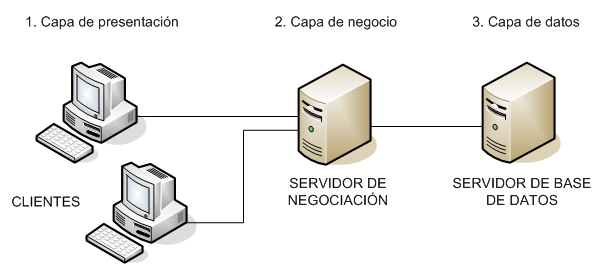
\includegraphics[width=15cm]{images/image12}
\centering
\caption[]{Arquitectura 3 capes.}
\centering
\end{figure}

\subsection{Tecnologia utilitzada}
Per la implementació del software, hem utilitzat una sèrie de tecnologies, frameworks i llenguatges de programació. Aquestes tecnologies es llisten a continuació.

\subsubsection{HTML5}

HTML, o Hyper Text Markup Language, és el llenguatge bàsic que s'utilitza per estrocturar documents web. És un llenguatge d'etiquetes que permet definir diferents elements en una pàgina web. Aquests elements poden se botons, enllaços, imatges, text plà, o qualsevol tipus d'element que ens ajudi a crear una pàgina web.

\subsubsection{CSS}

CSS, o Cascading Style Sheets, és un llenguatge de fulls d'estil que permet desriure la presentació (tant estil com format) d'un document basat en llenguatge d'etiquetes.

\subsubsection{Javascript}

Javascript és un llenguatge basat en prototipus. Aquest llenguatge, juntament amb la llibreria jQuery, ens serveixen per manipular elements de la pàgina web, o l'estil d'aquests, de forma dinàmica.

\subsubsection{Neo4j}

Neo4j és una base de dades no relacional, la qual es caracteritza per no tenir un esquema definit. És una graph database, el qual implica que la base de dades estarà definida per nodes i relacions entra aquests.\\ \\
En una aplicació com la que s'esta implementant ens és molt útil, ja que l'informació d'aquesta va fluctuant tota l'estona i les cerques sín més ràpides, ja que totes surten d'un node concret.

\subsubsection{JSON}
JSON, o Javascript Object Notation, és un llenguatge obert basat en text i orientat a l'intecanvi de dades. A més és facil d'entandre per qualsevol persona, inclús si aquesta no es troba en el món de la informàtica.\\ \\
Per agafar l'informació de la base de dades, necessitem implementar una API o un connector amb Javascript, de forma que aquest ens permeti tenir un flux d'informació. Per fer-ho, totes les queries de consulta que es fan retornen el seu resultat en en format JSON.

\subsubsection{Node.js}

És un framework que et facilita totes les feines encarades a web. Els seus llenguatges bàsics són HTML, CSS i Javascript, tot i que pots afegir les funcionalitats que vulguis instal·lant els paquets necessaris al teu projecte.\\ \\
Finalment, dir que aquest framework et dóna molta facilitat per implementar la comunicació client servidor.\\ \\
Els paquets addicionals que s'han utilitzat en l'aplicació són els següents:

\begin{itemize}
\item \textbf{body-parser:} Aquest paquet ens permet llegir els camps que ha omplert el client directament des del servidor, sense la necessitat d'haver de fer una crida ajax per passar els paràmetres.
\item \textbf{bootstrap:} És un framework per HTML, CSS i Javascript que permet fer les pàgines responsive amb facilitat.
\item \textbf{dotenv:} ens permet carregar fitxers .env a l'aplicació.
\item \textbf{jquery:} És una llibreria de Javascript que et permet escriure el mateix codi de forma més ràpida, i que permet la manipulació del codi HTML de forma senzilla.
\item \textbf{jquery-validation:} És un pluguin de jQuery que serveix per validar els diferents formularis que hi puguin haver a l'aplicació (dates, correus electrònics, contrasenyes, etc).
\item \textbf{neo4j-driver:} És un driver que permet configurar connexions amb Neo4j, ja explicat a l'apartat 3.3.
uuid: Ens permet auto generar un identificador únic per a cada node de la base de dades.
\item \textbf{pug:} Aquest paquet permet escriure el codi HTML més ràpidament i permet crear bucles d'informació dinàmica a la pàgina web.
\item \textbf{font-awesome:} És una llibreria d'icones.
\item \textbf{w3-css:} Permet fer dissenys més amistosos per l'usuari de l'aplicació amb facilitat.
\item \textbf{crypto:} Aquest paquet ens permet encriptar les contrasenyes dels usuaris, en base64, utilitzant diferents algoritmes.
\item \textbf{client-session:} Paquet que ens permetrà mantenir les sessions dels usuaris.
\item \textbf{multer:} Paquet que permet al client penjar fotografies al servidor utilitzant funcions middleware.
\item \textbf{moment:} Permet definir formats de dates.
\item \textbf{fullcalendar:} Permet visualitzar diferents esdeveniments en un calendari a partir d'un JSON.
\item \textbf{materialize-css:} Paquet que m'ha permés fer la interfície gráfica més amigable. Aquest paquet, conté una serie de classes css i funcions javascript que permeten tenir una millor interacció amb la UI de l'aplicació.

\end{itemize}

\subsubsection{Webstorm}

Webstorm és una IDE, creada per JetBrians, encarada al desenvolupament d'aplicacions web i que ens servirà per fer la implementació de la aplicació.\\ \\
Els seus llenguatges principals són Javascript, HTML i CSS.

\subsection{User Interface}

\subsubsection{Fonts}

L'aplicació estarà composta per dues fonts:
\begin{itemize}
\item \textbf{Montserrat:} És la font que s'utilitzarà en els títols.
\item \textbf{Raleway:} S'utilitzarà per a la resta de text de l'aplicació.
\end{itemize}
He triat aquestes fonts a partir de les guis d'estil de google (\url{https://fonts.google.com/}). Montserrat és la font que ens servirà pels títols, i Raleway com a font sans-serif, que és la que es recomana per la major part del text de la pàgina.

\subsubsection{Colors primaris de l'aplicació}

L'aplicació està composta per la següent paleta de colors:

\begin{figure}[h]

\includegraphics[width=12cm]{images/image1}
\centering
\caption[]{Paleta de colors de l'aplicació.}
\centering
\end{figure}
Per troba'ls, he utilitzat una eina que es diu \textbf{paletton}, la qual et permet combinar colors de forma senzilla. Per utilitzar-la podeu entrar a la següent URL:\\
\url{http://paletton.com/\#uid=5300u0kqALsd8VjkyQ8B3GbBuoR} \\ \\
Si us fixeu, en quasi totes les xares socials conegudes, s'utilitza el blau com a color principal de l'aplicació. Jo he decidit ficar el ver per trencar una mica els esquemes i que l'aplicació pugui ser facilment reconeguda.

\subsubsection{Logotip}

Per fer el logotip de l'aplicació, s'han utilitzat les mateixes fonts que s'han esmentat anteriorment.
El resultat és el següent:

\begin{figure}[H]

\includegraphics[width=7cm]{images/image3}
\centering
\caption[]{Logotip de l'aplicació.}
\centering
\end{figure}

El logotip, intenta representar una mà com a símbol representatiu de l'amistat. D'aquí el nom de MakeYourFriend.

\subsection{Mapes navigacionals}

A continuació, es mostren els dos mapes navigacionals, tant pels usuaris com pels administradors del sistema:

\begin{figure}[H]
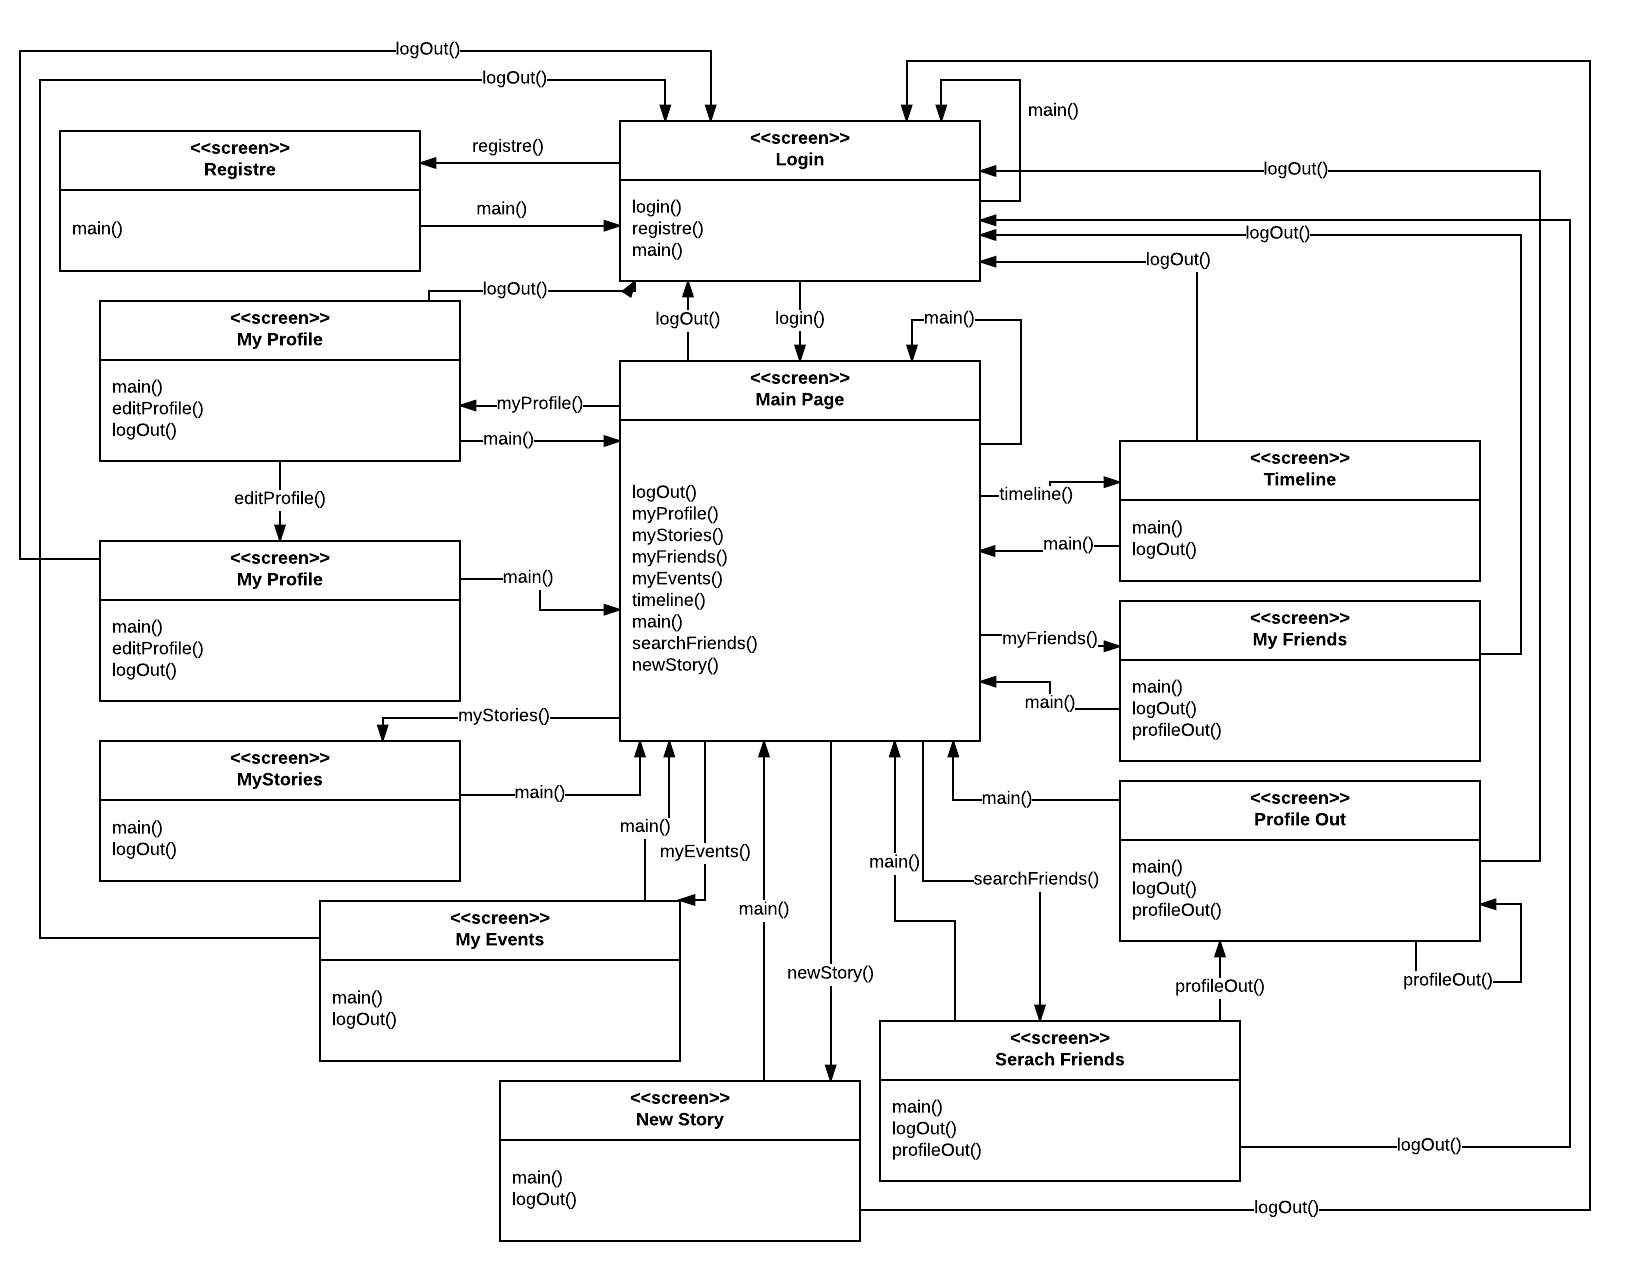
\includegraphics[width=11cm]{images/image9}
\centering
\caption[]{Mapa navigacional de l'aplicació (Usuari).}
\centering
\end{figure}

\begin{figure}[H]
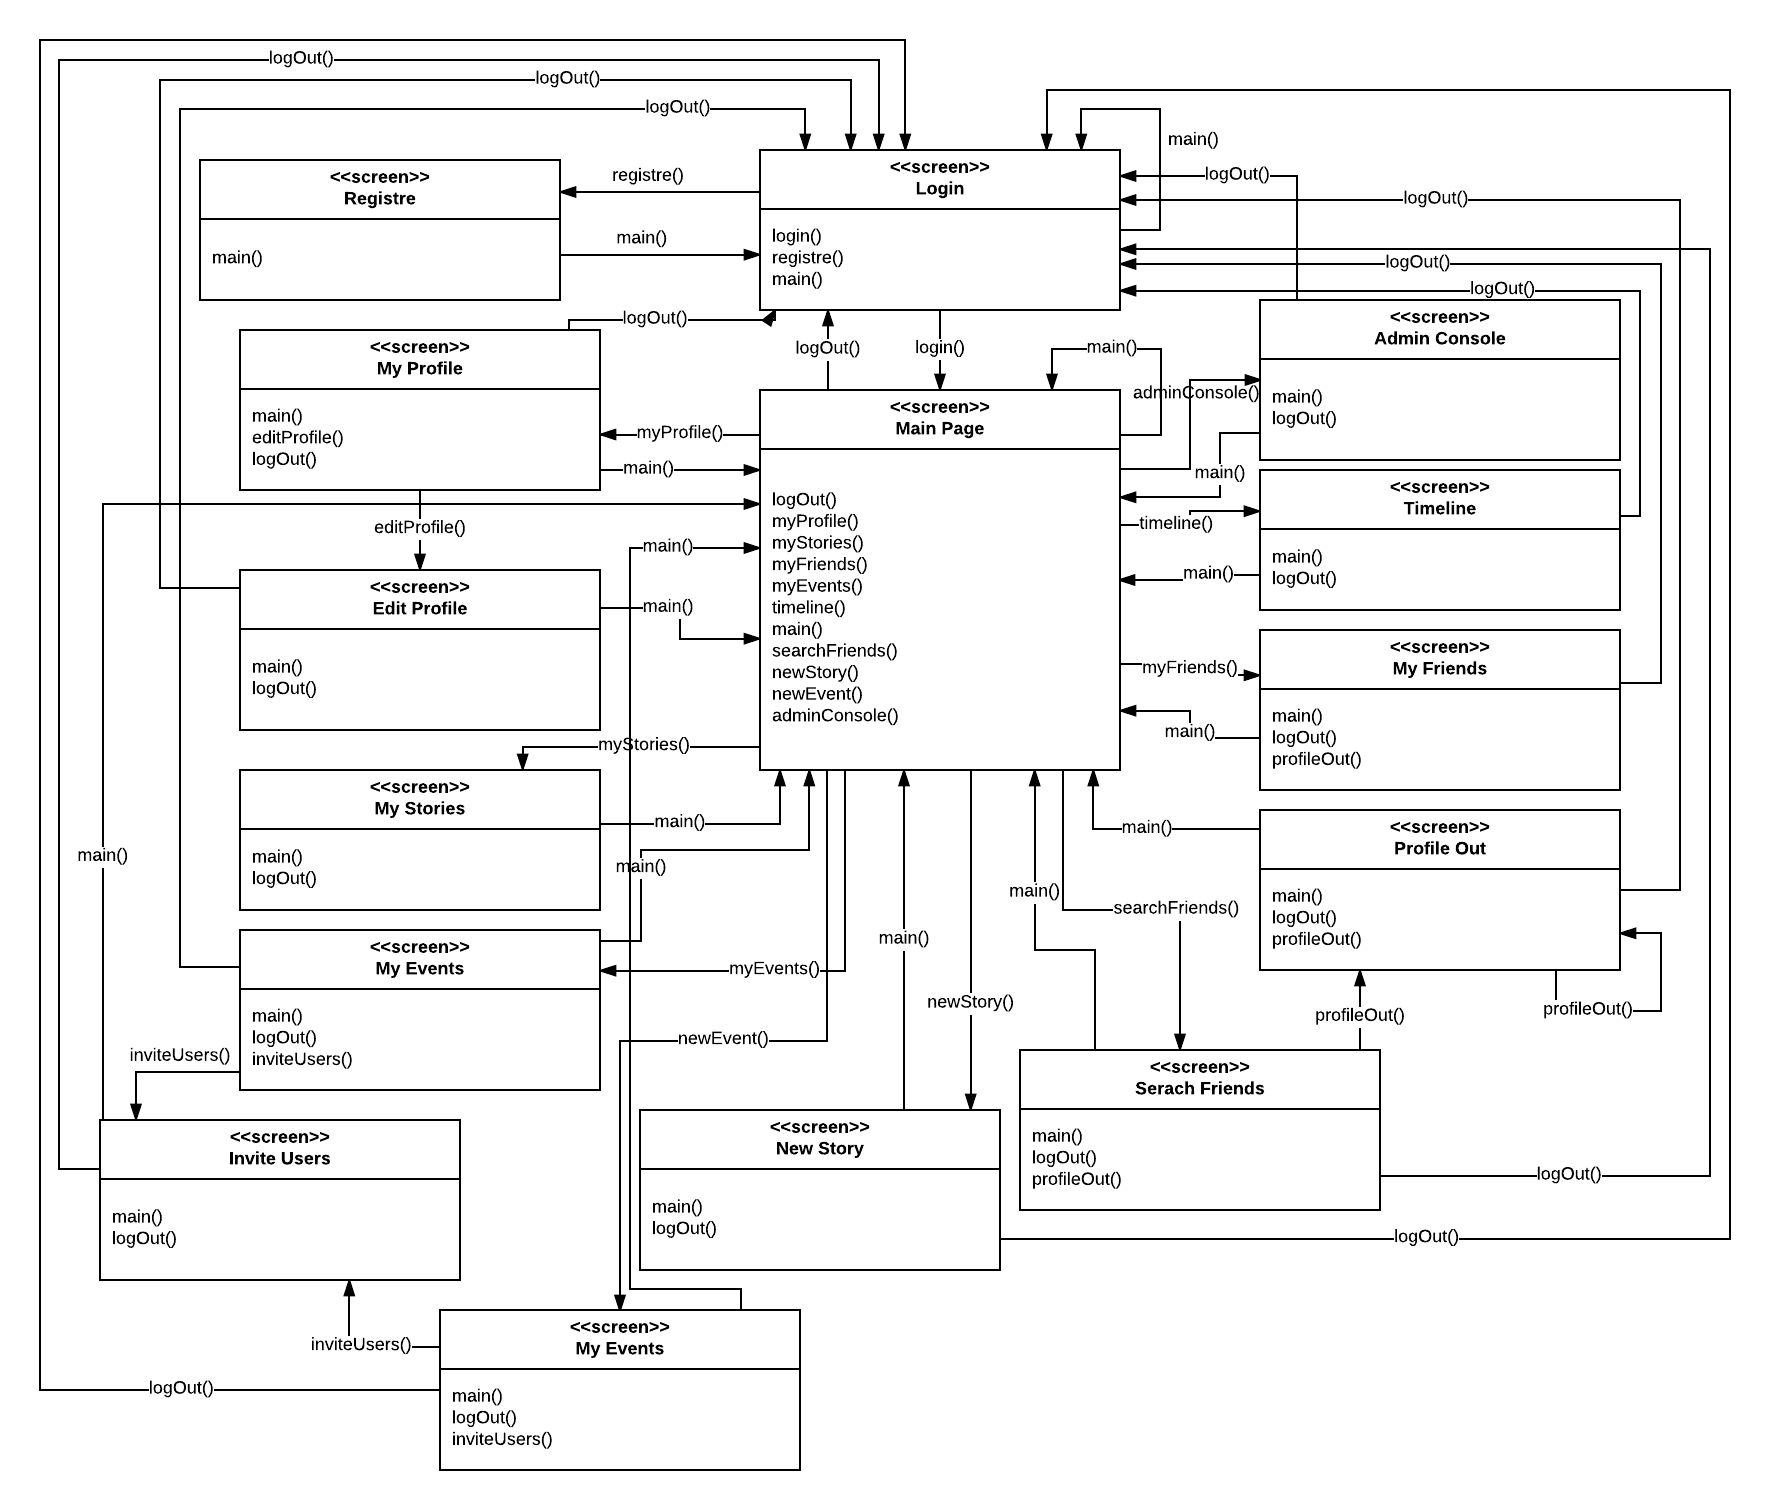
\includegraphics[width=15cm]{images/image10}
\centering
\caption[]{Mapa navigacional de l'aplicació (Gestor/Administrador).}
\centering
\end{figure}

\subsection{Model de dades}

Com hem dit anterirment, en la base de dades que s'utilitzan no hi ha un esquema definit. Tot hi aixó, s'han definit unes entitats i unes relacions entre aquestes per mantindre una constancia de la informació. Les entitats són les següents:

\begin{figure}[h]
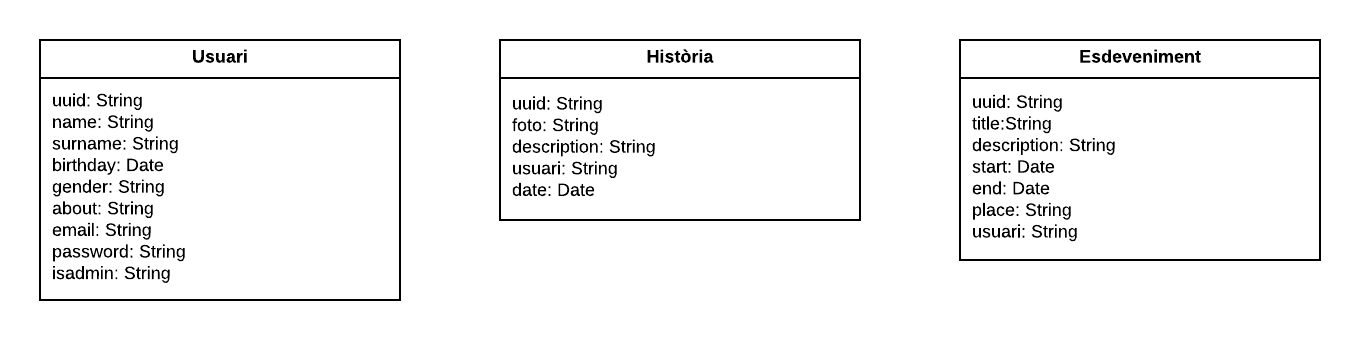
\includegraphics[width=15cm]{images/image6}
\centering
\caption[]{Entitats de l'aplicació.}
\centering
\end{figure}

\subsubsection{Usuari}

L'usuari representa tant els usuaris del sistema com el seu gestor/administrador. Els camps que té aquesta entitat són els següents:
\begin{itemize}
	\item \textbf{uuid:} Representa l'identificador únic dins de la base de dades.
	\item \textbf{name:} Conté el nom de l'usuari.
	\item \textbf{surname:} Conté el cognom o congnoms de l'usuari.
	\item \textbf{birthday:} Conté la data de naixament de l'usuari.
	\item \textbf{gender:}  Conté el gènere de l'usuari. El gènere pot ser "Male" o "Female".
	\item \textbf{about:} Conté la descripció de l'usuari. El que l'usuari vol que sàpiguin d'ell.
	\item \textbf{email:} Conté el correu electònic de l'usuari.
	\item \textbf{password:} Conté la contrasenya en base-64 de l'usuari.
	\item \textbf{isadmin:} Camp que informa de si l'usuari és administrador/gestor.
	\item \textbf{foto:} Conté la ruta on esta guardada la fotografia del seu perfil.
	\item \textbf{code:} Conté el codi d'administrador. Els usuaris necessiten un codi per poder registrar-se al sistema, i aquest camp conté el codi, el qual es correspon amb el uuid de l'administrador.
\end{itemize}

\subsubsection{Història}

Una història representa una publicació que l'usuari a fet dins del sistema. Aquesta publicació es guarda amb els següents camps:
\begin{itemize}
	\item \textbf{uuid:} Representa l'identificador únic dins de la base de dades.
	\item \textbf{foto:} Conté la ruta de la fotografia que l'usuari ha afegit a l'història. En cas que l'història no tingui cap foto, el camp es defineix amb "nothing".
	\item \textbf{description:} Conté la descripció de l'història.
	\item \textbf{usuari:} Conté el nom i el cognom de l'usuari que he fet la publicació. 
	\item \textbf{date:} conté la data en que s'ha creat l'història.
\end{itemize}

\subsubsection{Esdeveniment}
Un esdeveniment és una entitat en que els usuaris poden indicar si i volen assistir o no. Aquest esdeveniment conté els següents camps:
\begin{itemize}
	\item \textbf{uuid:} Representa l'identificador únic dins de la base de dades.
	\item \textbf{title:} Conté el títol de l'esdeveniment.
	\item \textbf{description:} Conté la descripció de l'esdeveniment.
	\item \textbf{start:} Conté el dia i l'hora d'inici de l'esdeveniment.
	\item \textbf{end:} Conté el dia i l'hora de finalització de l'esdeveniment.
	\item \textbf{place:} Conté el lloc on es durà a terme l'esdeveniment.
	\item \textbf{usuari:} Conte el nom i el congom de l'usuari que ha creat l'esdeveniment.
\end{itemize}
Tot i tenir les entitats, no podem contenir totes les dades del sistema, ja que aquestes entitats només contenen informació d'una unitat única dins de l'aplicació. Per aixó, s'han definit diferents relacions entre les entitats del sistema. Per a que es puguin entendre les diferents relacions, s'utilitzarà el llenguatge Cypher, que és el llenguatge de queries que s'utilitza en la bases de dades neo4j. Les relacions es definiràn de la següent manera:
\begin{itemize}
	\item \textbf{(exemple):} Els parentesis indiquen que és un node, i exemple representaria el nom del node.
	\item \textbf{-[exemple]->:} -[]-> representa una relació d'un node a un altre, i exemple seria el nom de la relació.
\end{itemize}
Les relacions que tenim dins del sistema són les següents:
\begin{itemize}
	\item \textbf{(Usuari A)-[MY\_FRIEND]->(Usuari B):} Aquesta relació representa que l'usuari A té amistat amb l'usuari B. Com que neo4j no permet una relació bidireccional, si en el sistema trobem una relació MY\_FRIEND d'un node a un altre, implica que existirà la mateixa relació en sentit contrari.
	\item \textbf{(Usuari A)-[MY\_REQUEST]->(Usuari B):} Aquesta relació representa que l'usuari A ha solicitat tenir amistat amb l'usuari B. Si existeix aquesta relació, implica que l'usuari A no pot tenir una relació de MY\_FRIEND (explicada anteriorment) amb l'usuari B i a l'inversa.
	\item \textbf{(Usuari A)-[MY\_POST]->(Post A):} Aquesta relació indica que el Post A (Història A) ha estat creada per l'usuari A.
	\item \textbf{(Usuari A)-[LIKE]->(Post A):} Aquesta relació indica que a l'usuari A li agrada el Post A (Història A).
	\item \textbf{(Usuari A)-[MY\_EVENT]->(Esdeveniment A):} Aquesta relació indica que l'esdeveniment A ha estat creat per l'usuari A.
	\item \textbf{(Esdeveniment A)-[EVENT\_REQUEST]->(Usuari A):} Aquesta relació indica que l'usuari A esta convidat a l'esdeveniment A.
	\item \textbf{(Usuari A)-[ASSIST\_EVENT]->(Esdeveniment A):} Aquesta relació indica que l'usuari A assistirà a l'esdeveniment A.
\end{itemize}

Per acabar aquesta secció, la imatge següent mostra un exemple (molt reduït) de la base de dades:

\begin{figure}[H]
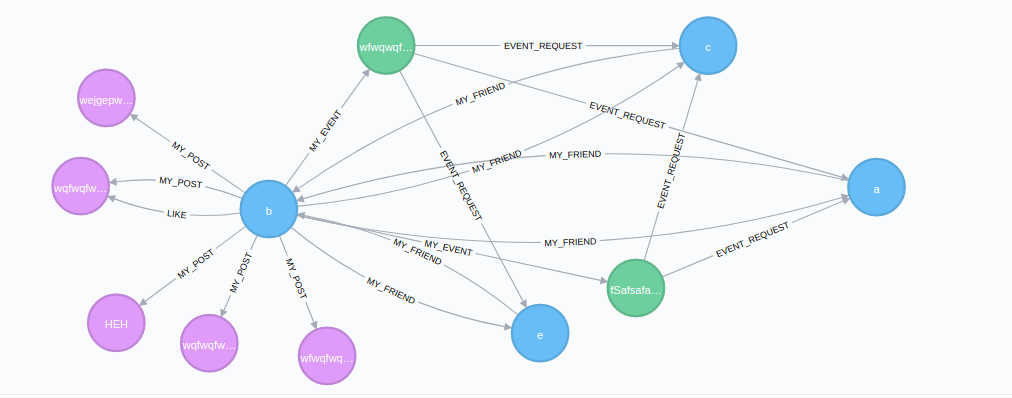
\includegraphics[width=15cm]{images/image11}
\centering
\caption[]{Exemple reduït de la base de dades}
\centering
\end{figure}
Els nodes de color rosa represente històries, els de color verd esdeveniments, i els de color blau els usuaris del sistema.

\section{Implementació}
En aquest apartat, es donaràn exemples de codi de les funcions principals del sistema.

\subsection{Sessions}
Per implementar les sessions, s'ha utilitzat el paquet de Node.js anomenat client-session. Per fer que les sessions siguin estables, s'ha passat a través d'una cookie tota la informació correponent al node de l'usuari, i seguidament, per cada request de l'usuari al servidor, es valida si la cookie es valida. Per fer-ho s'ha procedit de la següent manera:
\begin{enumerate}
	\item En primer lloc s'importa la llibreria en una variable:
		\begin{lstlisting}
			const session = require('client-sessions');
		\end{lstlisting}
	\item Seguidament, configurem les cookies:
\begin{lstlisting}
app.use(session({
  cookieName: 'session',
  secret: 'randomWord',
  duration: 30 * 60 * 1000,
  activeDuration: 5 * 60 * 1000,
}));	
\end{lstlisting}
A la cookie, i afegim un nom i el temps de duració.
\item Una vegada la cookie esta configurada, aquesta s'ha de passar al client en el moment que fa login:
\begin{lstlisting}
function setLogin(email, password, res, req, page, pageer) {
  db.findUser(email).then((usr) => {
    if (!usr[0]) {
      res.render(pageer, { error: 'Invalid email or password.' });
    } else {
      const hash = crypto.createHash('sha256').update(password).digest('base64');
      if (usr[0].password == hash) {
        user = usr[0];
        req.session.usr = usr;
        res.redirect(page);
      } else {
        res.render(pageer, { error: 'Invalid email or password.' });
      }
    }
  });
}
\end{lstlisting}
Com podem veure, en primer lloc validem que l'usuari i la contrasenya siguin valids. Per fer-ho ens comuniquem amb la capa de dades (db en el codi), mirem si l'usuari existeix, i si és així, comprovem la seva contrasenya. En el cas que no sigui valid, redireccionem al login amb error, i en cas que sigui correcte el redireccionem a la pàgina principal i li passem la cookie amb tota la seva informació.
\item Una vegada l'usuari té la cookie, per cada crida que fa al servidor s'executa la següent funció:
\begin{lstlisting}
function requireLogin(req, res, next) {
  if (!req.session.usr) {
    if (req.get('accept-language').includes('ca')) {
      res.redirect('/login-ca');
    } else if (req.get('accept-language').includes('es')) {
      res.redirect('/login-es');  
    } else res.redirect('/login-en');
  } else {
    next();
  }
}
\end{lstlisting}
En el cas que la cookie ja no sigui vàlida (tant per que la cookie ha caducat, com que s'ha tancat el navegador), es redirecciona a la pàgina d'inici de l'aplicació (el login). Altrament, navegarà a la pàgina que l'usuari hagi demanat.
\end{enumerate}
Tot el codi d'aquest apartat, es troba en el fitxer app.js.

\subsection{Registre}
En aquest apartat, es donarà com exemple com s'ha fet el registre d'un nou usuari. Per fer-ho, s'han fet servir uns quants fitxers, els quals s'aniràn anomenant pas a pas:
\newpage
\begin{enumerate}
	\item Per poder registrar un usuari al sistema, s'ha d'omplir el següent formulari, corresponent al fitxer que es troba en la ruta /views/register/register-en:
\begin{figure}[h]
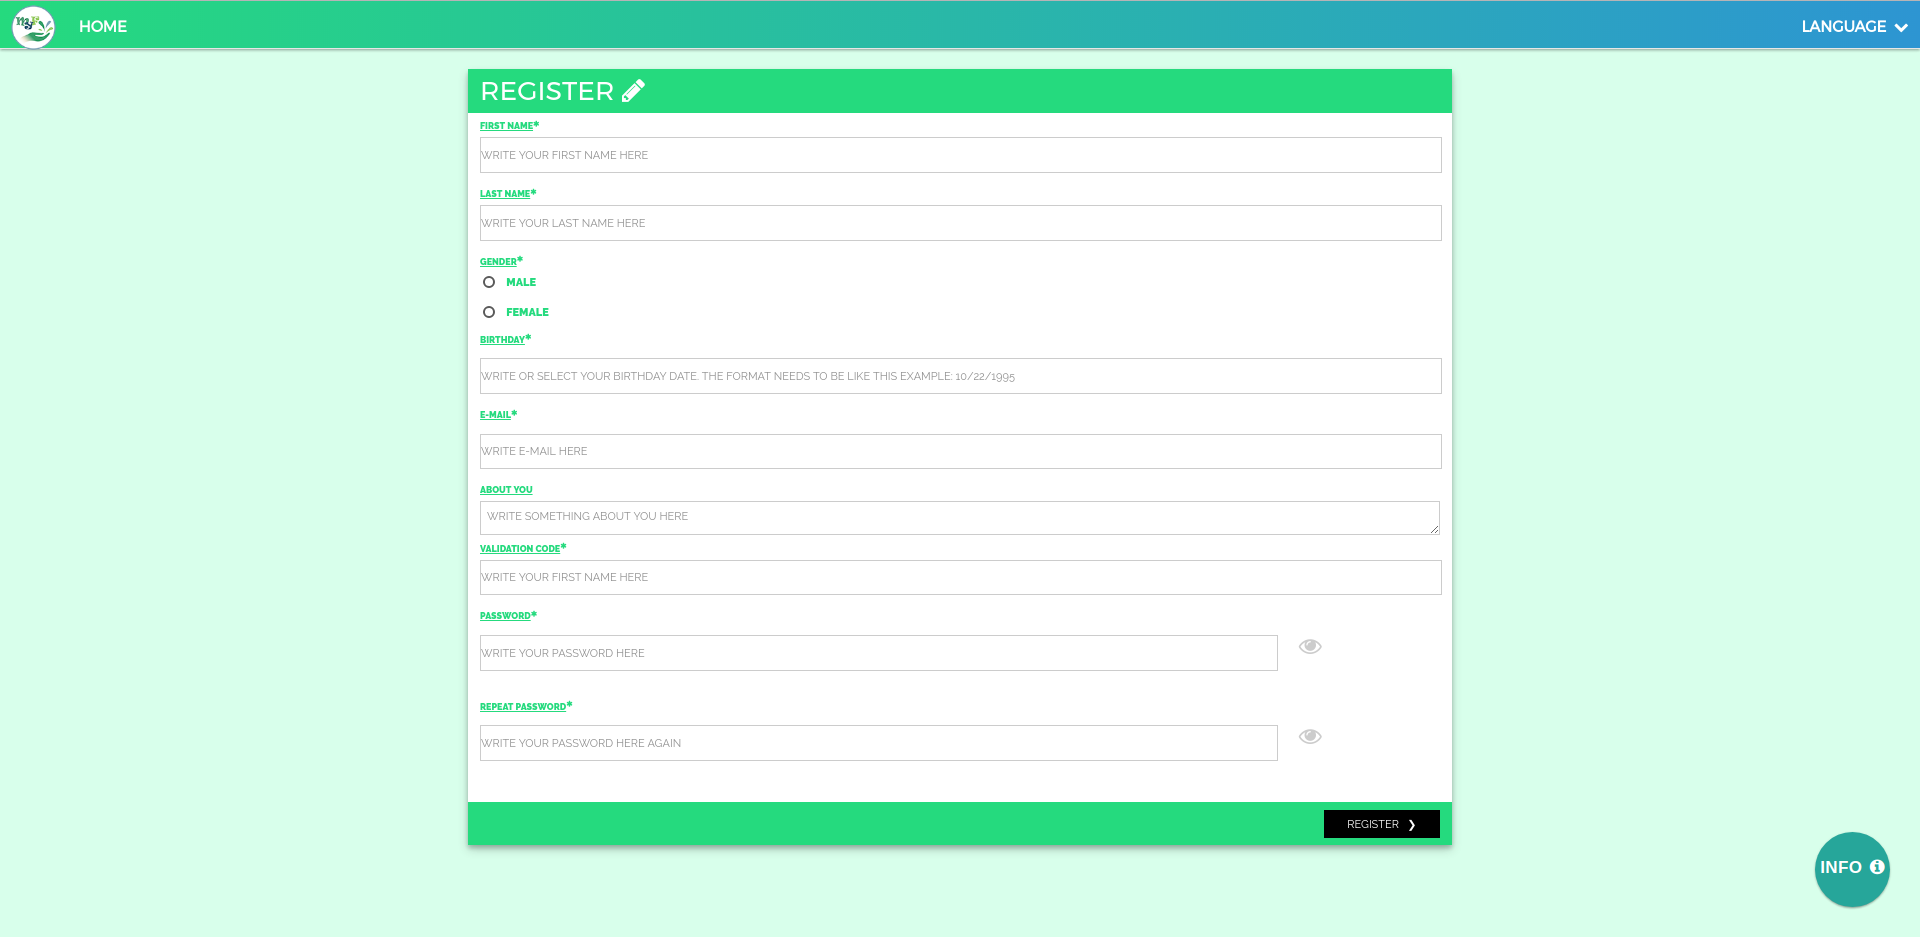
\includegraphics[width=15cm]{images/image13}
\centering
\caption[Figura 3.1]{Pàgina de registre.}
\centering
\end{figure}
\item Una vega s'omple el formulari i es clica el botó register, s'executa el següent codi (que es troba en el mateix fitxer):
\begin{lstlisting}
$( "#submitbutton" ).click(function() {
        var form = $("#registerform");
        form.validate({
            rules: {
                email: {
                    required: true,
                    email: true
                },
                pass1: {
                    required: true,
                    minlength: 8
                },
                pass2: {
                    required: true,
                    equalTo: "#pass1"
                },
                birthday:{
                    isValidDate: true
                }
            }
        });

        if(form.valid()) {
            $('#spinnerbackground').css('display', 'block');
            $('#spinner').css('display', 'block');
            $.ajax({
                url: "/getUsers"
            }).done(function (users) {
                var exists = false;
                var validCode = false;
                for(i=0;i<users.length;++i){
                    if(users[i].email == document.getElementsByName("email")[0].value){
                        exists = true;
                        i=users.length;
                    }
                    if(users[i].uuid.toLowerCase() == document.getElementsByName("code")[0].value.toLowerCase() && users[i].isadmin=="YES"){
                        validCode = true;
                    }
                }
                if (exists) {
                    $('#spinnerbackground').css('display', 'none');
                    $('#spinner').css('display', 'none');
                    $('#infobackground').css('display', 'block');
                    $('#errorcard').css('display', 'block');
                }
                else {
                    if(validCode == false){
                        $('#spinnerbackground').css('display','none');
                        $('#spinner').css('display', 'none');
                        $('#infobackground').css('display', 'block');
                        $('#errorcardcode').css('display', 'block');
                    }
                    else form.submit();
                }
            }).fail(function () {
                $('#spinnerbackground').css('display', 'none');
                $('#spinner').css('display', 'none');
            });
        }
    });
\end{lstlisting}
Com podem veure, en primer lloc, es valida que el formulari s'hagi omplert correctament. Seguidament s'executa una query per agafar tots els usuaris del sistema. Aquesta query, anirà al fitxer app.js (capa de negoci) i seguidament al fitxer neo4j-api.js (capa de dades), Agafarà els usuaris del sistema i els mostrarà al client. A partir d'aquí, es validarà que el codi de validació introduit per l'usuari sigui vàlid i que l'usuari no existeixi al sistema.
\item Si el codi de validació no és vàlid, l'usuari haurà de tornar d'omplir el camp de codi d'usuari. Altrament, es farà submit del formulari i s'executarà la petició post de /registe-en, en l'arxiu app.js (el qual conté totes les rutes de l'aplicació.):
\begin{lstlisting}
app.post('/register-en', (req, res) => {
  const name = req.body.name;
  const surname = req.body.surname;
  const gender = req.body.gender;
  const code = req.body.code;

    // FORMAT TO STANDAR DATE
  const auxDate = req.body.birthday;
  const parts = auxDate.split('/');
  const birthday = `${parts[1]}/${parts[0]}/${parts[2]}`;

  const email = req.body.email.toLowerCase();
  const about = req.body.about;
  const password = req.body.pass1.toLowerCase();

  db.createUser(name, surname, gender, birthday, email, about, password, code)
        .then(() => res.redirect('/login-en?fromreg=YES'))
        .catch(error => res.status(500).send(error));
});
\end{lstlisting}
\item Com es pot veure agafem tots els parametres del formulari, es fan les transformacions pertinents i finalment, executem la funció db.createUser, la qual es troba en el fitxer neo4j-api.js:
\begin{lstlisting}
  createUser(name,surname,gender,birthday,email,about,password,code){
    var isadmin = "NO";

    const session = this.driver.session();

    const hash = crypto.createHash('sha256').update(password).digest('base64');

    const resp = session
        .run(`
          CREATE (n:USER {
            name: {name},
            surname: {surname},
            gender: {gender},
            birthday: {birthday},
            email: {email},
            about: {about},
            code: {code},
            password: {hash},
            uuid: {uuid},
            isAdmin: {isadmin}
          })
          RETURN n.name`, {
          name,
          surname,
          gender,
          birthday,
          email,
          about,
          code,
          hash,
          uuid: uuid(),
          isadmin
        });

    resp.then(() => session.close())
        .catch(() => session.close());

    return resp;
  }
\end{lstlisting}
Aquesta funció encripta la contrasenya en un hash en base64, i seguidament, executa una query a la base de dades (vindria a ser session.run()). Una vegada s'ha executat la query, es retorna el resultat, i com s'ha vist al metode post del fitxer app.js, en cas que la query hagi fallat, et retorna l'error 500. En el cas que l'usuari s'hagi creat correctament, et redireccionarà a la pantalla de login.
\end{enumerate}

\subsection{New Story}
Aquesta funcionalitat, dona l'oportunitat de poder penjar una història a l'usuari en qüestió. Per poder implementar-ho, s'ha seguit els següents passos:
\newpage
\begin{enumerate}
\item En primer lloc, s'ha creat un formulari el qual l'usuari ha d'omplir:
\begin{figure}[h]
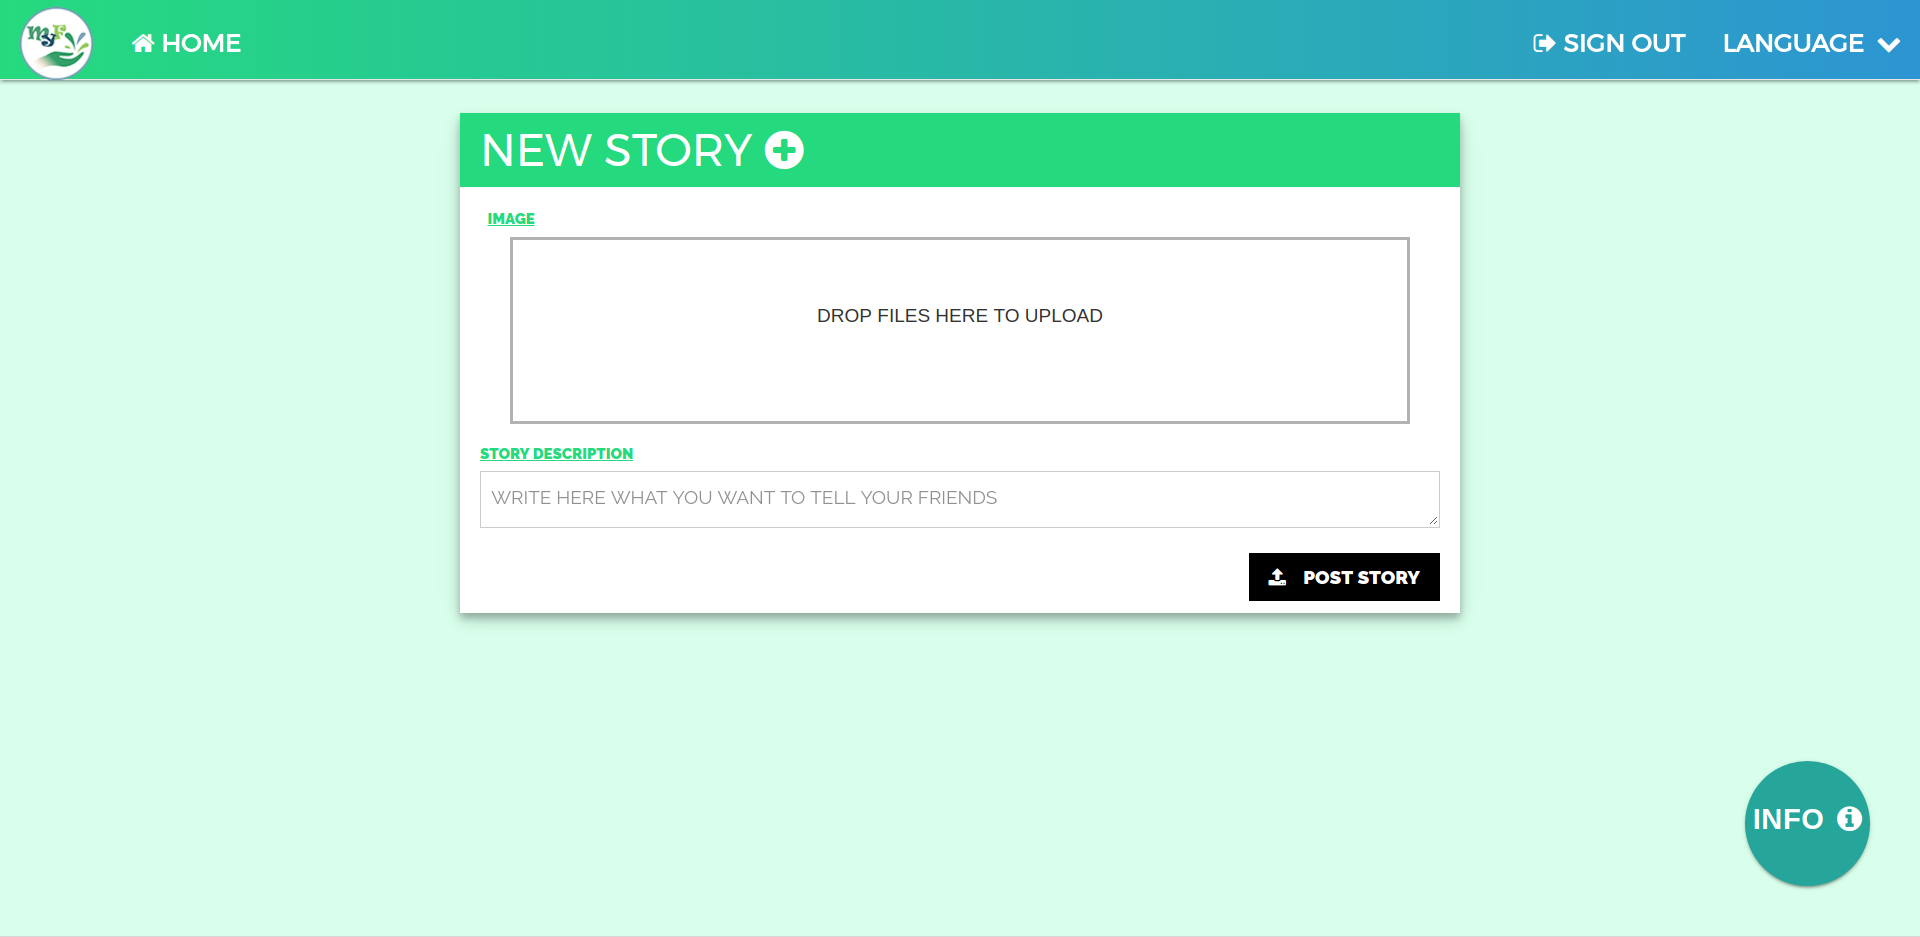
\includegraphics[width=15cm]{images/image14}
\centering
\caption[Figura 3.1]{Pàgina de New Story.}
\centering
\end{figure}
Com podem veure, podem penjar una imatge i podem ficar una descripció. Per poder penjar la imatge (fent ús del drag \& drop), s'ha procedit de la següent forma:
\begin{enumerate}
\item S'ha definit un formulari amb la classe dropzone i amb identificador \#imageform en el fitxer /views/new-post/new-post-en:
\begin{lstlisting}
form#imageform.dropzone.w3-container(action="/post-image", method="post", enctype="multipart/form-data")
   label.w3-text(style="margin-top:-45px;margin-left:-40px !important;")
       b(style='text-decoration:underline;') IMAGE
\end{lstlisting}
\item Una vegada s'ha definit el formulari, es defineix el dropzone en el mateix fitxer:
\begin{lstlisting}
Dropzone.options.imageform = {

        // Prevents Dropzone from uploading dropped files immediately
        autoProcessQueue: false,
        maxFiles: 1,
        addRemoveLinks: true,
        init: function () {
            var submitButton = document.querySelector("#submitbutton")
            myDropzone = this; // closure

            submitButton.addEventListener("click", function () {
                var form = $("#registerform");
                if(form.valid()) {
                    $('#spinnerbackground').css('display', 'block');
                    $('#spinner').css('display', 'block');
                    myDropzone.processQueue();
                    if (myDropzone.getUploadingFiles().length === 0 && myDropzone.getQueuedFiles().length === 0) {
                        var description = $("#description").val();
                        console.log(description);
                        $.ajax({
                            method: "POST",
                            url: "/post-story/" + description,
                            success: function () {
                                var form = $("#registerform");
                                form.submit();
                            }
                        });
                    }
                }
            });

            myDropzone.on("complete", function(file) {
                if (this.getUploadingFiles().length === 0 && this.getQueuedFiles().length === 0) {
                    var description = $("#description").val();
                    console.log(description);
                    $.ajax({
                        method: "POST",
                        url: "/post-story/" + description,
                        success: function () {
                            var form = $("#registerform");
                            form.submit();
                        }
                    });
                }
            });
        }
    };
\end{lstlisting}
En aquesta definició, es pot veure que una vegada es cliqui el submit button, es pujarà la imatge al servidor (només en el cas que aquesta existeixi).
\item Quan l'imatge es puja al servidor, s'utilitza la següent ruta:
\begin{lstlisting}
app.post('/post-image', uploadPost.single('file'), (req, res) => {
    res.send('OK');
});
\end{lstlisting}
La qual executa la funció uploadPost.single('file') definida de la següent forma:
\begin{lstlisting}
const storagePost = multer.diskStorage({
  destination: './uploadsPost/',
  filename(req, file, cb) {
    crypto.pseudoRandomBytes(16, (err, raw) => {
      if (err) return cb(err);
      lastUpload = `./uploadsPost/${raw.toString('hex')}${path.extname(file.originalname)}`;
      fileUploaded = true;
      cb(null, raw.toString('hex') + path.extname(file.originalname));
    });
  }
});

var maxSize = 1 * 1000 * 1000*1000*1000;

const uploadPost = multer({
    storage: storagePost,
    limits: { fileSize: maxSize },
});
\end{lstlisting}
Una vegada s'ha pujat la imatge al servidor, es segueix amb la l'execució del codi per publicar l'história.
\end{enumerate}
\item Com hem dit anteriorment, una vegada la imatge s'ha pujat al servidor (en el cas que aquesta existeixi), es fa una nova crida al servidor:
\begin{lstlisting}
app.post('/post-story/:description', requireLogin, (req, res) => {
      const description = req.params.description;
      const date = new Date();
      const dateInMilliseconds = date.getTime();
      const usuari = `${req.session.usr[0].name} ${req.session.usr[0].surname}`;
      console.log("ehehehehehhehehe");
      if(fileUploaded===true){
          console.log("1");
          db.newPost(req.session.usr[0].email, description, lastUpload, dateInMilliseconds, usuari).then(() => {
              console.log("POST");
              db.relationToNewPost(req.session.usr[0].email, dateInMilliseconds);
          });
          console.log("LOG");
      }
      else{
          console.log("2");
          db.newPost(req.session.usr[0].email, description, 'nothing', dateInMilliseconds, usuari).then(() => {
              console.log("POST");
              db.relationToNewPost(req.session.usr[0].email, dateInMilliseconds);
          });
          console.log("LOG");
      }
      fileUploaded=false;
      res.send('OK');
});
\end{lstlisting}
En aquesta crida es distingeix si anteriorment s'ha pujat una imatge al servidor. Si és així, aquesta es passa com a parametre a la funció newPost de la capa de dades. Altrament, aquest parametre es passa com a 'nothing'. Finalment, es fa una nova crida a la capa de dades (relationToNewPost), la qual permet crear una relació MY\_POST, entre l'usuari i la nova història. Les dos operacions són les següents:
\begin{itemize}
\item \textbf{newPost():}
\begin{lstlisting}
  newPost(email,description,foto, date, usuari){
      const session = this.driver.session();

      const resp = session
          .run(`CREATE (n:POST {
            description: {description},
            foto: {foto},
            date: {date},
            usuari: {usuari},
            uuid: {uuid}
            }) RETURN n.uuid`, {
              description,
              foto,
              date,
              usuari,
              uuid: uuid(),
          });

      resp.then(() => session.close())
          .catch(()=> session.close());

      return resp;
  }
\end{lstlisting}
\item \textbf{relationToNewPost():}
\begin{lstlisting}
relationToNewPost(email,date){
      const session = this.driver.session();

      var time = new Date().getTime();
      var query = "MATCH (u:USER), (r:POST) WHERE u.email = '"+email+"' AND r.date = "+date+" CREATE (u)-[t:MY_POST {date:'"+time+"'}]->(r) RETURN t";

      const resp = session.run(query);

      resp.then(()=> session.close())
          .catch(()=> session.close());

      return resp;
  }
\end{lstlisting}
\end{itemize}
\item Per acabar, es fa una última crida al servidor, la qual redireccionarà al client a la pàgina d'inici.
\begin{lstlisting}
app.post('/redirect-after-post', requireLogin, (req, res) => {
    res.redirect('/main-page-en');
});
\end{lstlisting}
\end{enumerate}

\subsection{Other User Profile}
Aquesta funcionalitat permet poder veure el perfil d'un altre usuari. A diferencia de les funcinalitats anteriors, aquesta funcionalitat es correspon a un get del fitxer app.js.\\ \\
Per fer-ho s'ha procedit de la següent forma:
\begin{enumerate}
\item En primer lloc, l'usuari fa la següent creda get al servidor:
\begin{lstlisting}
app.get('/profile-out-en/:targetEmail', requireLogin, (req, res) => {
  const email = req.params.targetEmail;
  if (email == req.session.usr[0].email) res.redirect('/profile-en');
  else {
    db.findUser(email).then((result) => {
      const usuari = result[0];
      db.getFriends(email).then((result2) => {
        const friends = result2;
        db.getMyStories(email,req.session.usr[0].email).then((result3) => {
          const posts = result3;
          db.getIfFriend(email,req.session.usr[0].email).then((result4) => {
              var isFriend = false;
              if(result4[0]!=null) isFriend=true;
              res.render('./profile-out/profile-out-en.pug', { usuari, friends, posts,isFriend});
          });
        });
      });
    });
  }
});
\end{lstlisting}
En primer lloc, comprovem que el perfil que volem veure no sigui el nostre. En cas que el perfil sigui el nostre, s'enrutarà a l'usuari al app.get("profile-en"), que es correspon a la ruta de del nostre perfil. Seguidament fem les següents crides a la capa de dades:
\begin{itemize}
\item \textbf{findUser():}
\begin{lstlisting}
findUser(email){
      const session = this.driver.session();

      const promise = new Promise((resolve, reject) => {
          session
              .run(`MATCH (s:USER) WHERE s.email = "` + email + `" RETURN s`)
              .then((result) => {
                  session.close();
                  resolve(result.records
                      .map(record => record._fields[0].properties));
              })
              .catch((error) => {
                  session.close();
                  reject(error);
              });
    });

    return promise;
  }
\end{lstlisting}
\item \textbf{getFriends():}
\begin{lstlisting}
    getFriends(myemail){
        const session = this.driver.session();

        var query = "MATCH (n:USER {email: '"+myemail+"'})-[:MY_FRIEND]->(p:USER) RETURN p";

        const promise = new Promise((resolve,reject) => {
            session.run(query)
                .then((result) => {
                    session.close();
                    resolve(result.records
                        .map(record => record._fields[0].properties));
                })
                .catch((error) => {
                    session.close();
                    reject(error);
                });
        });

        return promise;
    }
\end{lstlisting}
\item \textbf{getMyStories():}
\begin{lstlisting}
  getMyStories(email,myemail){
      const session = this.driver.session();

      var query = `MATCH (n:USER {email: "`+email+`"})-[:MY_POST]->(p:POST), (r:USER {email: "`+myemail+`"})
              SET p.likes = SIZE(()-[:LIKE]->(p))
              SET p.liked = SIZE((r)-[:LIKE]->(p))
              RETURN p`;

      const promise = new Promise((resolve, reject) => {
          session
              .run(query)
              .then((result) => {
                  session.close();
                  resolve(result.records
                      .map(record => record._fields[0].properties));
              })
              .catch((error) => {
                  session.close();
                  reject(error);
              });
      });
      return promise;
  }
\end{lstlisting}
\item \textbf{getIfFriend():}
\begin{lstlisting}
  getIfFriend(target,myemail){
      const session = this.driver.session();

      var query = "MATCH (n:USER {email: '"+myemail+"'})-[r:MY_FRIEND]->(p:USER {email:'"+target+"'}) RETURN r";

      const promise = new Promise((resolve,reject) => {
          session.run(query)
              .then((result) => {
                  session.close();
                  resolve(result.records
                      .map(record => record._fields[0].properties));
              })
              .catch((error) => {
                  session.close();
                  reject(error);
              });
      });

      return promise;
  }
\end{lstlisting}
\end{itemize}
\item Una vegada que s'ha agafat la informació necessaria de la capa de dades, es renderitza la pàgina web que el client vol veure passant-li tota aquets informació.
\end{enumerate}

\section{Proves}
Les proves que s'han dut a terme per validar el software, són UT (Unit Test). Els Unit Test, són un tipus de proves que consisteixen en realitzar proves els components més petits de la nostra aplicació, ho sigui, es testeja cada una de les funcionalitats del sistema de forma indivudial.\\ \\
Addicinalment, per garantir més rigidesa de l'aplicació, el testeig ha estat realitzat, en part, per companys que també es trabaven fent el TFG.

%%%%%%%%%%%%%%%%%%%%%%%%%%%%%%%%%%%%%%%%%%%%%%%%%%%%%%%%%%%%%%%%%%%%%%%%%%%%%%%
%                                 CONCLUSIONS                                 %
%%%%%%%%%%%%%%%%%%%%%%%%%%%%%%%%%%%%%%%%%%%%%%%%%%%%%%%%%%%%%%%%%%%%%%%%%%%%%%%

\chapter{Conclusions}

????? ????????????? ????????????? ????????????? ????????????? ????????????? 

%%%%%%%%%%%%%%%%%%%%%%%%%%%%%%%%%%%%%%%%%%%%%%%%%%%%%%%%%%%%%%%%%%%%%%%%%%%%%%%
%                                BIBLIOGRAFIA                                 %
%%%%%%%%%%%%%%%%%%%%%%%%%%%%%%%%%%%%%%%%%%%%%%%%%%%%%%%%%%%%%%%%%%%%%%%%%%%%%%%

\begin{thebibliography}{10}

%%%%%%%%%%%%%%%%%%%%%%%%%%%%%%%%%%%%%%%%%%%%%%%%%%%%%%%%%%%%%%%%%%%%%%%%%%%%%%%
% MODEL D'URL                                                                 %
%%%%%%%%%%%%%%%%%%%%%%%%%%%%%%%%%%%%%%%%%%%%%%%%%%%%%%%%%%%%%%%%%%%%%%%%%%%%%%%
\bibitem{WAR}
   Discapacitat cognitiva.
   \newblock Consultat a 
   \url{https://neeitic.jimdo.com/part-te\%C3\%B2rica/discapacitats/discapacitat-cognitiva/}.

\bibitem{WAR}
   Xarxa social - Viquipèdia, l'enciclopèdia lliure.
   \newblock Consultat a 
   \url{https://ca.wikipedia.org/wiki/Xarxa_social}.
   
\bibitem{WAR}
   Historia de las redes sociales - Recursos - Ministerio de Educación.
   \newblock Consultat a 
   \url{http://recursostic.educacion.es/observatorio/web/es/internet/web-20/1043-redes-sociales?start=2}.

\bibitem{WAR}
   Bulletin Board System - Viquipèdia, l'enciclopèdia lliure.
   \newblock Consultat a 
   \url{https://ca.wikipedia.org/wiki/Bulletin_Board_System}.

\bibitem{WAR}
   Aplicaciones para niños con Necesidades Educativas Especiales ....
   \newblock Consultat a 
   \url{http://www.chaval.es/chavales/educacion/aplicaciones-para-ni\%C3\%B1os-con-necesidades-educativas-especiales}.

\bibitem{WAR}
   Stimulus – APP profesional de estimulación cognitiva.
   \newblock Consultat a 
   \url{http://stimuluspro.com/}.

\bibitem{WAR}
   10 apps para alumnos con dificultades específicas de aprendizaje.
   \newblock Consultat a 
   \url{http://www.educaciontrespuntocero.com/accesibilidad/apps-alumnos-dificultades-especificas-aprendizaje-dea/25080.html}.

\bibitem{WAR}
   Twitter - Viquipèdia, l'enciclopèdia lliure.
   \newblock Consultat a 
   \url{https://ca.wikipedia.org/wiki/Twitter}.

\bibitem{WAR}
   Facebook - Viquipèdia, l'enciclopèdia lliure.
   \newblock Consultat a 
   \url{https://ca.wikipedia.org/wiki/Facebook}.

\bibitem{WAR}
   Instagram - Viquipèdia, l'enciclopèdia lliure.
   \newblock Consultat a 
   \url{https://ca.wikipedia.org/wiki/Instagram}.

\bibitem{WAR}
   LinkedIn - Viquipèdia, l'enciclopèdia lliure.
   \newblock Consultat a 
   \url{https://ca.wikipedia.org/wiki/LinkedIn}.
   
\bibitem{WAR}
   Chart: Facebook Users Show No Signs of Tiring | Statista.
   \newblock Consultat a 
   \url{https://www.statista.com/chart/5380/facebook-user-engagement/}.

\end{thebibliography}
\cleardoublepage


%%%%%%%%%%%%%%%%%%%%%%%%%%%%%%%%%%%%%%%%%%%%%%%%%%%%%%%%%%%%%%%%%%%%%%%%%%%%%%%
%                              FI DEL DOCUMENT                                %
%%%%%%%%%%%%%%%%%%%%%%%%%%%%%%%%%%%%%%%%%%%%%%%%%%%%%%%%%%%%%%%%%%%%%%%%%%%%%%%

\end{document}
